\documentclass[10pt,a4paper,openright]{book}

%% Formateo del título del documento
\title{Topología elemental}
\author{Mario Calvarro Marines}
\date{}

%% Formateo del estilo de escritura y de la pagina
\pagestyle{plain}
\setlength{\parskip}{0.35cm} %edicion de espaciado
\setlength{\parindent}{0cm} %edicion de sangría
\clubpenalty=10000 %líneas viudas NO
\widowpenalty=10000 %líneas viudas NO
\usepackage[top=2.5cm, bottom=2.5cm, left=3cm, right=3cm]{geometry} % para establecer las medidas de los margenes
\usepackage[spanish]{babel} %Para que el idioma por defecto sea español
\usepackage{ulem} % para poder subrayar entornos especiales como las secciones

%% Texto matematico y simbolos especiales
\usepackage{amsmath} %Paquetes para mates
\usepackage{mathtools}
\usepackage{amsfonts} %Paquetes para mates
\usepackage{amssymb} %Paquetes para mates
\usepackage{stmaryrd} % paquete para mates
\usepackage{latexsym} %Paquetes para mates
\usepackage{cancel} %Paquete tachar cosas
\usepackage{accents} %Paquete acentos

%% Ruta de las fotos e inclusion de las mismas
\usepackage{graphicx}
\graphicspath{{./fotos/}}

%% Inclusion de referencias cruzadas por defecto y específicas
\usepackage{hyperref}

%% Paquete para definir y utilizar colores por el documento
\usepackage[dvipsnames,usenames]{xcolor} %activar e incluir colores
    %% definicion de los colores que se van a utilizar en cada cabecera
    \definecolor{capitulos}{RGB}{60,0,0}% gama de colores de los capitulos
    \definecolor{secciones}{RGB}{95,8,5}% gama de colores de las secciones
    \definecolor{subsecciones}{RGB}{140,36,31}% gama de colores de las subsections
    \definecolor{subsubsecciones}{RGB}{188,109,79}% gama de colores de las subsubsections
    \definecolor{teoremas}{RGB}{164,56,32}% gama de colores para los teoremas
    \definecolor{demos}{RGB}{105,105,105} % gama de colores para el cuerpo de las demostraciones

%% Paquete para la edición y el formateo de capítulos, secciones...
\usepackage[explicit]{titlesec}
    %% Definición del estilo de los capítulos, secciones, etc...
    \titleformat{\chapter}[display]{\normalfont\huge\bfseries\color{capitulos}}{}{0pt}{\Huge #1}[\titlerule]
    \titleformat{\section}{\normalfont\Large\bfseries\color{secciones}}{}{0pt}{#1}
    \titleformat{\subsection}{\normalfont\large\bfseries\color{subsecciones}}{}{0pt}{\uline{#1}}
    \titleformat{\subsubsection}{\normalfont\normalsize\bfseries\color{subsubsecciones}}{}{0pt}{#1}

%% Paquete para el formateo de entornos del proyecto
\usepackage{ntheorem}[thmmarks]
    %% Definicion del aspecto de los entornos matematicos del proyecto
    \theoremstyle{break}
    \theoremheaderfont{\normalfont\bfseries\color{teoremas}}
    \theorembodyfont{\itshape}
    \theoremseparator{\vspace{0.2cm}}
    \theorempreskip{\topsep}
    \theorempostskip{\topsep}
    \theoremindent0cm
    \theoremnumbering{arabic}
    \theoremsymbol{}
    \theoremprework{\vspace{0.2cm} \hrule}
    \theorempostwork{\vspace{0.2cm}\hrule}
        \newtheorem*{defi}{Definición}

    \theoremprework{\vspace{0.25cm}}
        \newtheorem*{theo}{Teorema}

    \theoremprework{\vspace{0.25cm}}
    	\newtheorem*{coro}{Corolario}

    \theoremprework{\vspace{0.25cm}}
    	\newtheorem*{lema}{Lema}

    \theoremprework{\vspace{0.25cm}}
    	\newtheorem*{prop}{Proposición}

    \theoremheaderfont{\normalfont}
    \theorembodyfont{\normalfont\color{demos}}
    \theoremsymbol{\hfill\square}
    	\newtheorem*{demo}{\underline{Demostración}:}

    \theoremheaderfont{\normalfont}
    \theorembodyfont{\normalfont}
    	\newtheorem*{obs}{\underline{Observación}:}
    	\newtheorem*{ej}{\underline{Ejemplo}:}
    	\newtheorem*{pg}{\underline{Política general}:}
    	\newtheorem*{il}{\underline{Ilustración}:}

%% Definicion de operadores especiales para simplificar la escritura matematica
\DeclareMathOperator{\dom}{dom}
\DeclareMathOperator{\img}{img}
\DeclareMathOperator{\rot}{rot}
\DeclareMathOperator{\divg}{div}
\DeclareMathOperator{\inter}{Int}
\DeclareMathOperator{\adh}{Adh}
\DeclareMathOperator{\fr}{Fr}
\newcommand{\dif}[1]{\ d#1}

%% Paquete e instrucciones para la generacion de los dibujos
\usepackage{pgfplots}
\pgfplotsset{compat=1.17}
\usepackage{tkz-fct}
\usepgfplotslibrary{fillbetween}
\usepackage{tikz,tikz-3dplot}
\tdplotsetmaincoords{80}{45}
\tdplotsetrotatedcoords{-90}{180}{-90}
\usetikzlibrary{arrows}
    %% style for surfaces
    \tikzset{surface/.style={draw=blue!70!black, fill=blue!40!white, fill opacity=.6}}

    %% macros to draw back and front of cones
    %% optional first argument is styling; others are z, radius, side offset (in degrees)
    \newcommand{\coneback}[4][]{
        %% start at the correct point on the circle, draw the arc, then draw to the origin of the diagram, then close the path
        \draw[canvas is xy plane at z=#2, #1] (45-#4:#3) arc (45-#4:225+#4:#3) -- (O) --cycle;
    }
    \newcommand{\conefront}[4][]{
        \draw[canvas is xy plane at z=#2, #1] (45-#4:#3) arc (45-#4:-135+#4:#3) -- (O) --cycle;
    }
    
    \tikzset{middlearrow/.style={decoration={markings, mark= at position 0.5 with {\arrow{#1}},},postaction={decorate}}}
    
    \usetikzlibrary{decorations.markings}
    
    \newcommand{\AxisRotator}[1][rotate=0]{
    \tikz [x=0.25cm,y=0.60cm,line width=.2ex,-stealth,#1] \draw (0,0) arc (-150:150:1 and 1);
    }
    
    \usetikzlibrary{shapes}


\begin{document}
\maketitle
\setcounter{tocdepth}{3}% para que salgan las subsubsecciones en el indice
\tableofcontents
\chapter{Espacios topológicos}%
\label{cha:espacios_topologicos}

\section{Conjuntos abiertos}%
\label{sec:conjuntos_abiertos}
\begin{defi}
Una \underline{topología} en un conjunto $X$ es una colección $\mathcal{T} \subset \mathcal{P}\left( x \right)$ de subconjuntos tal que:
\begin{enumerate}
    \item $\emptyset, X \in \mathcal{T}$ 
    \item Las uniones arbitrarias de elementos de $\mathcal{T}$ están en $\mathcal{T}$.
    \item Las intersecciones \underline{finitas} de elementos de $\mathcal{T}$ están en $\mathcal{T}$.
\end{enumerate}
Se dice que $\left( X, \mathcal{T} \right)$ es un \underline{espacio topológico}, los elementos de $\mathcal{T}$ se llaman \underline{abiertos} y los elementos de $X$ se llaman \underline{puntos}. 
\end{defi}

\begin{ej}
\begin{enumerate}
    \item \label{ejemplos_topologia:first} $\mathcal{T} = \{\emptyset, X\}$ es la topología \underline{trivial}; $\mathcal{T} = P\left( X \right)$, topología \underline{discreta}: si los puntos $\{x\} \in \mathcal{T}$, entonces cualquier $A = \bigcup_{x \in A} \{x\}$ es abierto.
    \item $\mathbb{R}^n$ con la topología usual definida mediante las bolas euclídeas.
    \item Cualquier distancia $d$ define una topología mediante sus bolas abiertas, igual que se define la usual. \underline{Notación}: 
    \[
    B\left( a, \varepsilon \right) = \{d\left( a, x \right) < \varepsilon\},\ B\left[ a, \varepsilon \right] = \{d\left( a, x \right) \le \varepsilon \},\ S\left[ a, \varepsilon \right] = \{d\left( a, x \right) = \varepsilon\} 
    \]
    \item En un conjunto se pueden definir muchas topologías distintas (por ejemplo (\ref{ejemplos_topologia:first})) pero se puede asumir que solo ``parezcan'' distintas. Ya se sabe que la topología usual de $\mathbb{R}^n$ se puede definir mediante muchas distancias distintas.

    %TODO: Dibujo
    \begin{center}
        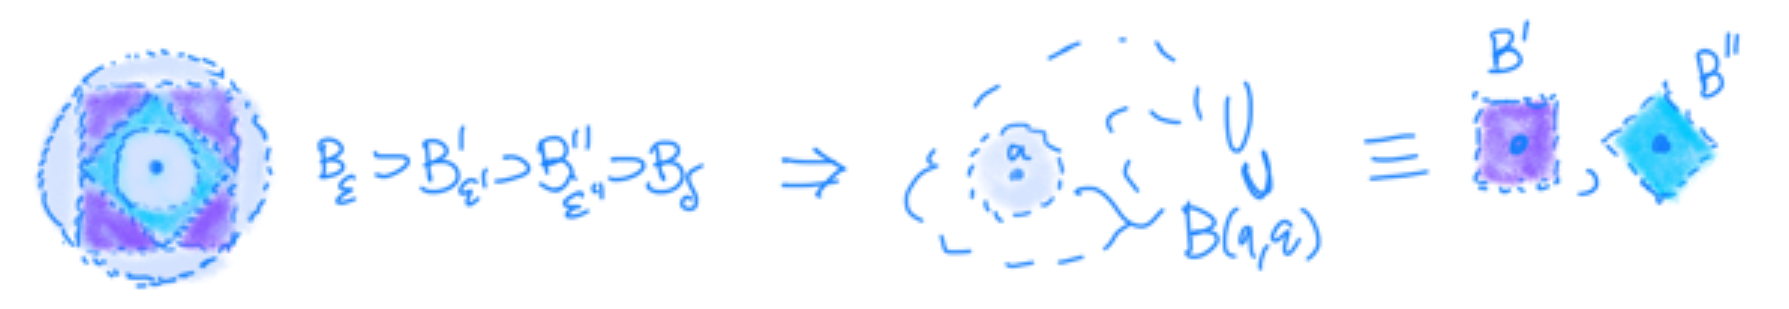
\includegraphics[scale=0.2]{images/topologia_metricas}  

        \textit{El dibujo representa distintas distancias\footnote{Procedentes de \textit{normas}.} en $\mathbb{R}^n$, pero todas definen la misma topología.} 
    \end{center}
    \item Una topología para ilustrar muchas propiedades (y contraejemplos). 

    Fijamos $a \in X$:
    \[
    \mathcal{T}_a = \{U \subset X: a \in U\} \cup \{\emptyset\} 
    \]
    La topología ``del punto''. El punto $\{a\}$ y todos los pares de puntos $\{a, x\}$ son abiertos. Se parece a la discreta pero difiere en que en esta última todos los puntos son abiertos.
\end{enumerate}
\end{ej}

\begin{defi}
Dos topologías $\mathcal{T}_1 \subset \mathcal{T}_2$ en $X$ se llaman \underline{comparables}: $\mathcal{T}_2$ es más ``fina'' que $\mathcal{T}_1$.
\end{defi}
Siempre se da:
\[
\mathcal{T}_{\text{trivial}} \subset \mathcal{T} \subset \mathcal{T}_{\text{discreta}} 
\]
Sea $\left( X, \mathcal{T} \right)$ un espacio topológico; a menudo se omite $\mathcal{T}$ ó el calificativo ``topológico''. 

\begin{defi}
\begin{enumerate}
    \item Un \underline{entorno abierto} de un punto $x \in X$ es un abierto $U$ que lo contiene. Se suele escribir $U^x$.
    \item Un \underline{entorno} de un punto $x \in X$ es un conjunto $V$ que contiene un abierto $U$ que contiene al punto. Se suele escribir $V^x$.\footnote{La intersección finita de entornos es entorno. (Si son abiertos es trivial)}
\end{enumerate}
\end{defi}
%TODO: Fix imagen
\begin{center}
    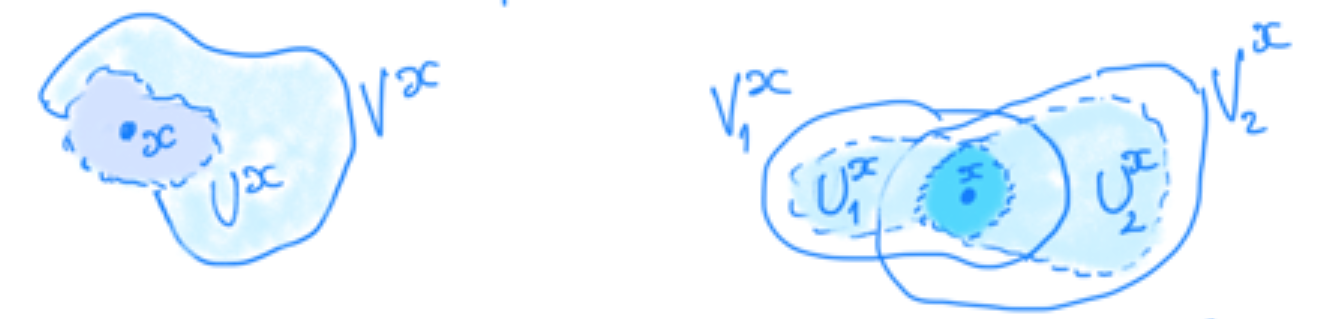
\includegraphics[scale=0.2]{images/def_entornos} 
\end{center}
\begin{obs}    
\begin{enumerate}
    \item Con $U^x \subset V^x$:
    \begin{align*}
        V_1^x \cap V_2^x &= V^x\\
        U_1^x \cap U_2^x &= U_{\text{ab}}^x \ni x
    \end{align*}

    %TODO: Corregir esta observación
    \item $U \in \mathcal{T}$ es entorno de todos \underline{sus} puntos.
    \begin{demo}
    \[
    x \in U \text{ abierto} \subset U
    \]
    \end{demo}
\end{enumerate}
\end{obs}

\begin{defi}
Sea $A \subset X$. Un \underline{punto interior de $A$} es un punto del que $A$ es entorno (luego $A$ lo contiene). El \underline{interior de $A$} es el conjunto de sus puntos interiores:
\[
\inter_X \left( A \right) = \mathring{A} = \{x \in A: \exists U_{\text{ab}}^x \subset A\} 
\]
\end{defi}
%TODO: Fix imagen
\begin{center}
    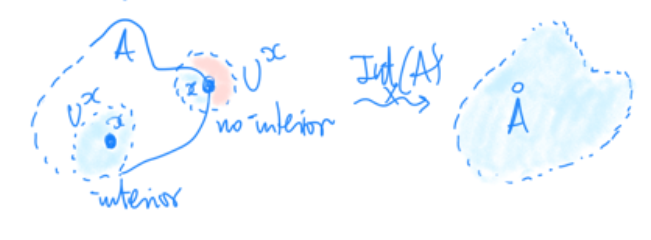
\includegraphics[scale=0.4]{images/def_interior} 
\end{center}

\begin{prop}
$\mathring{A}$ es el mayor abierto contenido en $A$: 
\[
\mathring{A} = \bigcup_{U^{ab} \subset A} U
\]
En particular, $A$ abierto $\Leftrightarrow A = \mathring{A} \Leftrightarrow A$ es un entorno de todos los puntos.    
\end{prop}
\begin{demo}
\begin{enumerate}
    \item $\mathring{A}$ es abierto: 
    \begin{gather*}
        \begin{rcases}
        \forall x \in \mathring{A} &\Rightarrow \exists U_{\text{ab}}^x \subset A\\
        \forall y \in U^x &\Rightarrow A \supset U^x \text{ es un abierto que contiene a } y \Rightarrow y \in \mathring{A}.\\
        \end{rcases} \Rightarrow U^x \subset \mathring{A}\\
        \Rightarrow \mathring{A} = \bigcup_{x \in \mathring{A}} U^x \text{ es abierto como unión de abiertos}
    .\end{gather*}
    \item $\mathring{A}$ es el mayor abierto contenido en $A$.
    \[
    U^{\text{ab}} \subset A \Rightarrow \forall x \in U^{\text{ab}} \subset A \Rightarrow x \in \mathring{A} \Rightarrow U \subset \mathring{A} 
    \]
\end{enumerate}
\end{demo}

\begin{ej}
\begin{enumerate}
    \item $\left( X, \mathcal{T}_{\text{trivial}} \right): A \neq X \Rightarrow A \not \supset X \Rightarrow \emptyset$ es el único abierto $\subset A \Rightarrow \mathring{A} = \emptyset$.

    \item En $\mathbb{R}^n$ con $\mathcal{T}_{\text{trivial}}$ ya lo sabemos bien:
    \[
    \inter\left( B\left[ a, \varepsilon \right] \right)  = B\left( a, \varepsilon \right);\ \mathring{\mathbb{Q}}^n = \emptyset;\ \mathring{\mathbb{Z}}^n = \emptyset
    \]
    \item Si $a \in X,\ \mathcal{T}_a : \mathring{\{a\}} = \{a\};\ x \neq a,\ \mathring{\{x\}} = \emptyset$.
\end{enumerate}
\end{ej}

\begin{prop}
\begin{enumerate}
    \item $A \subset B \Rightarrow \mathring{A} \subset \mathring{B}$.
    \item $\mathring{A} \cap \mathring{B} = \inter \left( A \cap B \right)$.
\end{enumerate}
\end{prop}
\begin{demo}
\begin{enumerate}
    \item $A \subset B \Rightarrow \mathring{A} \subset A \subset B$ y $\mathring{A}$ es abierto $\Rightarrow \mathring{A} \subset \mathring{B}$.
    \item 
    \begin{gather*}
    \begin{rcases}
    \begin{cases}
        \mathring{A} \cap \mathring{B} \text{ abierto (intersección finita de abiertos)}\\
        \mathring{A} \cap \mathring{B} \subset A \cap B 
    \end{cases} &\Rightarrow \mathring{A} \cap \mathring{B} \subset \inter \left( A \cap B \right)\\
    A \cap B \subset A, B \Rightarrow \inter \left( A \cap B \right) \subset \mathring{A}, \mathring{B} &\Rightarrow \inter\left( A \cap B \right) \subset \mathring{A} \cap \mathring{B}
    \end{rcases} \Rightarrow\\
    \boxed{\mathring{A} \cap \mathring{B} = \inter\left( A \cap B \right)} 
    .\end{gather*}
\end{enumerate}
\end{demo}

\section{Conjuntos cerrados}%
\label{sec:conjuntos_cerrados}
Sea $\left( X, \mathcal{T} \right)$ un espacio topológico.
\begin{defi}
Un conjunto \underline{cerrado} es un subconjunto $F \subset X$ tal que $U = X \setminus F$ es abierto.
\end{defi}
\begin{obs}
    Cerrado \underline{no} significa ``no abierto'', hay conjuntos que no son ni abiertos ni cerrados.
    %TODO: Fix imagen
    \begin{center}
        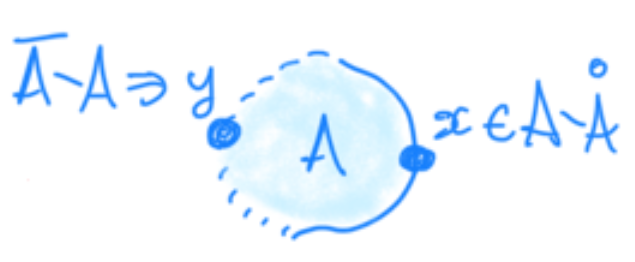
\includegraphics[scale=0.3]{images/def_cerrados} 
    \end{center}
\end{obs}
\begin{obs}
Se cumple, $\mathcal{F} = \{\text{cerrados}\}$:
\begin{enumerate}
    \item $X, \emptyset$ son cerrados.
    \item La intersección arbitraria de cerrados es cerrada.
    \item La unión finita de cerrados es cerrado.
\end{enumerate}
\begin{demo}
    Porque $\bigcap_{i \in  I} \left( X \setminus U_i \right) = X \setminus \bigcup_{i \in  I} U_i$ y $\bigcup_{i \in  I} X \setminus U_i = X \setminus \bigcap_{i \in  I} U_i$.
\end{demo}
\end{obs}

\begin{ej}
\begin{enumerate}
    \item En la topología trivial solo son cerrados $\emptyset$ y $X$. En la discreta, todos los subconjuntos son cerrados.
    \item En $\mathbb{R}^n$ con la topología usual ya sabemos todos los ejemplos: $B\left[ a, \varepsilon \right] : \lVert x - a \rVert \le \varepsilon$.
    \item Si $\mathcal{T}_1 \subset \mathcal{T}_2$, todo cerrado de $\mathcal{T}_1$ es cerrado de $\mathcal{T}_2$. (Cuidado con el orden) 
\end{enumerate}
\end{ej}

Para saber cuándo se aleja un conjunto de ser cerrado tenemos:
\begin{defi}
Sea $A \subset X$. Un punto \underline{adherente} a $A$ es un punto cuyos entornos intersecan todos a $A$. La \underline{adherencia} de $A$ es el conjunto de sus puntos adherentes. 
\[
\adh_X\left( A \right) = \overline{A} = \{x \in X: \forall V^x \cap A \neq \emptyset\} \supset A
\]
\end{defi}

\begin{obs}
Las primeras fórmulas importantes son:
\begin{gather*}
    \boxed{X \setminus \overline{A} = \inter\left( X \setminus A \right)} \\
    \boxed{X \setminus \mathring{B} = \overline{X \setminus B}} 
.\end{gather*}
\begin{demo}
\begin{itemize}
    \item $x \in X \setminus \overline{A} \Leftrightarrow x \not\in \overline{A} \Leftrightarrow \exists U^x \cap A = \emptyset \Leftrightarrow \exists U^x \subset X \setminus A \Leftrightarrow x \in \inter\left( X \setminus A \right)$
    \item $x \not\in \mathring{B} \Leftrightarrow \nexists U^x \subset B \Leftrightarrow \forall U^x \cap \left( X \setminus B \right) \neq \emptyset \Leftrightarrow x \in \overline{X \setminus B}$.
\end{itemize}
\end{demo}
\end{obs}

\begin{prop}
$\overline{A}$ es el menor cerrado que contiene a $A$: 
\[
    \boxed{\overline{A} = \bigcap_{F_{\text{cerrado}} \supset A} F } 
\]

En particular, $A$ cerrado $\Leftrightarrow \overline{A} = A \Leftrightarrow A$ contiene todos sus puntos de adherencia.
\end{prop}
\begin{demo}
$\overline{A} = X \setminus \inter\left( X \setminus A \right) = X \setminus \underbrace{\bigcup_{U \subset X \setminus A} U = X \setminus \bigcup_{F \supset A}}_{F = X \setminus U} \left( X \setminus F \right) = \bigcap_{F \supset A} F$.
\end{demo}

\begin{obs}
Lo anterior nos implica:
\begin{itemize}
    \item $B \supset A \Rightarrow \overline{B} \supset B \supset A \Rightarrow \overline{B} \supset \overline{A}$.
    \item $\overline{A \cup B} = \overline{A} \cup \overline{B}$:
    \[
    \begin{cases}
        \overline{A\cup B} \supset A \cup B \supset \begin{cases}
            A\\B
        \end{cases} \Rightarrow \overline{A\cup B} \supset \begin{cases}
            \overline{A} \\ \overline{B} 
        \end{cases} \Rightarrow \overline{A\cup B} \supset \overline{A} \cup \overline{B}\\

        A \cup B \subset \overline{A} \cup \overline{B} \Rightarrow \overline{A\cup B} \subset \overline{A} \cup \overline{B} 
    \end{cases} 
    \]
    La última implicación por que es cerrado al ser la unión de dos cerrados.
\end{itemize}
\end{obs}

\begin{ej}
\begin{enumerate}
    \item En $\mathbb{R}^n, \mathcal{T}_{\text{usual}}: B\left[ a, \varepsilon \right] = \overline{B \left( a, \varepsilon \right)};\ \overline{\mathbb{Q}^n} = \mathbb{R}^n$.
    \item $a \in X, \mathcal{T}_a$
    \[
        \begin{cases}
        \overline{\{a\}} = X \left[ \forall x, \forall U^x \supset \{a, x\} \ni a \Rightarrow x \in \overline{\{a\}} \right]\\
        x \neq a, \overline{\{x\}} = \{x\} \left[ y\neq x \Rightarrow U^y = \{a, y\} \cap \{x\} = \emptyset \right] 
        \end{cases} 
    \]
\end{enumerate}
\end{ej}

\begin{defi}[Otros puntos especiales]    
\begin{enumerate}
    \item $x$ es un \underline{punto aislado} de $A$ si $\exists V^x \cap A = \{x\}$.
    \item $x$ es un \underline{punto de acumulación} de $A$ si $\forall V^x \cap A \setminus \{x\} \neq \emptyset$. Y, evidentemente,
    \[
    \overline{A} = \{\underbrace{\text{puntos aislados}}_{\subset A}\} \sqcup \{\underbrace{\text{puntos de acumulación}}_{\supset \overline{A} \setminus A}\} 
    \]
    \item $x$ es un \underline{punto frontera} de $A$ si es adherente a $A$ y a $X \setminus A$, o bien, si no es interior de $X \setminus A$ ni de $A$. La \underline{frontera} de $A$ es: 
    \[
    \fr\left( A \right) = \{x \in X: x \text{ es punto frontera de } A\} = \overline{A} \cap \overline{X \setminus A} = \overline{A} \setminus \mathring{A}     
    \]
\end{enumerate}
\end{defi}

\begin{ej}
\begin{enumerate}
    \item En $\mathbb{R}, \mathcal{T}_n$ todos los puntos de $\mathbb{Z}$ son aislados, $\fr\left( \mathbb{Z} \right) = \mathbb{Z}$.
    \item En $\mathbb{R}^n, \mathcal{T}_n: \fr\left( B\left( a, \varepsilon \right) \right) = \fr\left( B\left[ a, \varepsilon \right] \right) = S\left[ a, \varepsilon \right] : \lVert x - a \rVert = \varepsilon$.
    \item En $\mathcal{T}_{\text{discreta}}$ todos los puntos son aislados, todas las fronteras son vacías.
    \item $a \in X, \mathcal{T}_a: $
    \[
    \begin{cases}
        \fr\left( \{a\} \right) = \overline{\{a\}} \setminus \mathring{\{a\}} = X \setminus \{a\}\\
        x \neq a, \fr\left( \{x\} \right) = \overline{\{x\}} \setminus \mathring{\{x\}} = \{x\} 
    \end{cases} 
    \]
\end{enumerate}
\end{ej}

Ahora, un concepto importante:
\begin{defi}
$A \subset X$ es \underline{denso} si $\overline{A} = X$, o bien, todo punto es adherente a $A$, o bien, todo abierto $\left( \neq \emptyset \right)$ corta a $A$.
\end{defi}

\begin{ej}
\begin{enumerate}
    \item $\mathbb{Q} \subset \mathbb{R}, \mathcal{T}_{\text{usual}}; \mathbb{Q} \times \overbrace{\ldots}^{n} \times \mathbb{Q} \subset \mathbb{R}^n, \mathcal{T}_{\text{usual}}$ son densos.
    \item $\{a\}$ es denso en $\left( X, \mathcal{T}_a \right)$.
\end{enumerate}
\end{ej}

\section{Bases}%
\label{sec:bases}
Sea $X, \mathcal{T}$ un espacio topológico.
\begin{defi}
Una \underline{base de entornos} de $a \in X$ es una colección $\mathcal{V}^a$ de entornos de $a$, tal que todo entorno de $a$ contiene uno de la $\mathcal{V}^a$.
\end{defi}

\begin{obs}
No se supone ninguna propiedad especial, ni que sean abiertos. Veremos que la existencia de base de entornos con propiedades adicionales es una de las cosas que determinan el comportamiento de la topología.

Pero: $\forall \mathcal{V}^a$ se puede \underline{refinar} a una base $\mathcal{B}^a$ de entornos de abiertos. 
\[
\left[ \forall V^a \in \mathcal{V}^a \exists U^a \subset V^a \Rightarrow \mathcal{B}^a = \{U^a: V^a \in \mathcal{V}^a\} \text{ es base de entornos} \right]
\]
\end{obs}

\begin{pg}
    Bastan las bases de entornos para comprobar propiedades de todos los entornos.
\end{pg}

\begin{il}    
\begin{align*}
    a \in \overline{A} &\xLeftrightarrow{\text{def}} \forall W^a \text{ entorno }: W^a \cap A \neq \emptyset\\
   &\Longleftrightarrow \forall V^a \in \mathcal{V}^a: V^a\cap A \neq \emptyset 
.\end{align*}
\end{il}

\begin{ej}
\begin{enumerate}
    \item $\mathbb{R}^n, \mathcal{T}_{\text{usual}}: $
    \[
    \begin{cases}
    \mathcal{B}^a = \{B\left( a, \varepsilon \right): \varepsilon > 0\} \text{ base de entornos abiertos.}  \\
    \mathcal{V}^a = \{B\left[ a, \varepsilon \right]: \varepsilon > 0\} \text{ base de entornos cerrados.} 
    \end{cases} 
    \]
    \item $a \in X, \mathcal{T}_a : \mathcal{B}^a = \{\{a\}\}, \mathcal{B}^x = \{\{a, x\}\},\ x \neq a$.
\end{enumerate}
\end{ej}

\begin{defi}
Una \underline{base de abiertos} de $\mathcal{T}$ es una colección de abiertos $B \subset \mathcal{T}$ tal que todo abierto es unión de abiertos de $B$.
\end{defi}

\begin{prop}
$\mathcal{B}$ base de abiertos $\Leftrightarrow \forall x \in X,\ \mathcal{B}^x = \{B \in \mathcal{B} : x \in B\}$ es base de entornos abiertos de $x \Leftrightarrow \forall x \in U,\ \exists B \in \mathcal{B} : x \in B \subset U$.
\end{prop}
\begin{demo}
$\Rightarrow) \forall V^x \Rightarrow x \in U \subset V^x \Rightarrow$
\[
    \mathcal{B} \text{ base } U = \bigcup_{i \in  I} \overbrace{B_i}^{\in \mathcal{B}} \xRightarrow{x \in U} \exists x \in B_i \subset U \subset V^x
\]
$\Leftarrow) U \in \mathcal{T},\ \forall x \in U,\ \exists \underbrace{B^x}_{\in \mathcal{B}} \subset U \Rightarrow U = \bigcup_{x \in U} B^x$ unión de abiertos de $\mathcal{B}$.
\end{demo}

\begin{ej}
\begin{enumerate}
    \item $\mathcal{T}_{\text{discreta}} : \mathcal{B} = \{\{x\} : x \in X\}$ es \underline{mínima}. $\left[ \text{si} B' \text{ es base } : \forall x, \{x\} = \bigcup_{i \in  I} \overbrace{B_i}^{\in B'} \Rightarrow B_i = \{x\} \right]$ 
    \item $\mathcal{T}_a: \mathcal{B} = \{\{a, x\} : x \in X\}$.
    \item $\mathbb{R}^n, \mathcal{T}_{\text{usual}} \mathcal{B} = \{B\left( x, \varepsilon \right) : \varepsilon > 0, x \in \mathbb{R}^n\}$
    %TODO: Fix imágenes 
    \begin{center}
        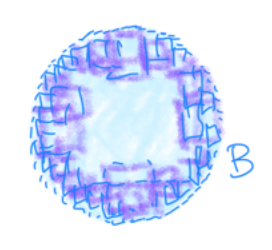
\includegraphics[scale=0.3]{images/base_rn} 
    \end{center}
    Pero también,
    \begin{center}
        
\includegraphics[scale=0.3]{images/bases_alternativas_rn} 
    \end{center}
    porque
    \[
    B\left( x, \varepsilon \right) = \bigcup_{i \in  I} cuadrados = \bigcup_{j \in J} rectangulos
    \]
\end{enumerate}
\end{ej}

\begin{pg}
    Como antes, a menudo basta considerar los abiertos de $\mathcal{B}$ 
\end{pg}

\begin{il}
$A \subset X$ denso $\Leftrightarrow \forall B \in \mathcal{B}, B \cap A \neq \emptyset$.
\end{il}

\begin{prop}
$\mathcal{B} \subset \mathcal{P} \left( X \right)$ es base de una topología (única) $\mathcal{T}$ es $X$. Es equivalente a: 
\begin{itemize}
    \item $X = \bigcup_{B \in \mathcal{B}} B$.
    \item $\forall x \in B_1 \cap B_2,\ \exists B^x \subset B_1 \cap B_2$.
\end{itemize}
%TODO: Fix imagen
\begin{center}
    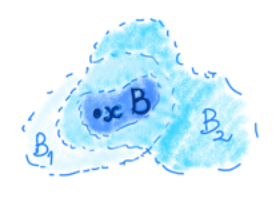
\includegraphics[scale=0.3]{images/base_unica} 
\end{center}
\end{prop}
\begin{demo}
\begin{itemize}
    \item \underline{Unicidad}: $\mathcal{T} = \{\bigcup_{i \in  I} B_i: \{B_i\} \subset \mathcal{B}\}$.
    \item \underline{Existencia}: Esa $\mathcal{T}$ es efectivamente topología. Lo importante: $B_1, B_2 \in \mathcal{B} \Rightarrow B_1 \cap B_2 = \bigcup_{x \in B_1 \cap B_2} B^x \in \mathcal{T}$.
\end{itemize}
\end{demo}

\section{Topología relativa}%
\label{sec:topologia_relativa}
Sea $\left( X, \mathcal{T} \right)$ espacio topológico.
\begin{defi}
$Y \subset X: \mathcal{T}|_Y = \{U \cap Y: U \in \mathcal{T}\}$ es una topología en $Y$ (fácil), denominada \underline{relativa} ó \underline{restricción} a $Y$; también se dice que $\left( Y, \mathcal{T}|_Y \right)$ es un \underline{subespacio} de $\left( X, \mathcal{T} \right)$ y que $\left( X, \mathcal{T} \right)$ es el espacio \underline{ambiente}. 
\begin{center}
    %TODO: Fix imagen
    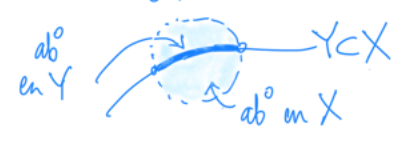
\includegraphics[scale=0.3]{images/def_subespacio_top} 
\end{center}
\end{defi}

\begin{obs}
\begin{enumerate}
    \item Los cerrados en $\mathcal{T}|_Y$ son $F\cap Y$ con $F$ cerrado en $\mathcal{T}$.
    \[
    \left[ Y \setminus U \cap Y = Y \cap \left( X \setminus U \right) = Y\cap F \right] 
    \]
    \item 
    $\begin{cases}
        y \in Y \subset X\\
        \mathcal{V}^y \text{ base de entornos de } y \text{ en } \mathcal{T} 
    \end{cases}\Rightarrow \begin{cases}
        \mathcal{V}^y \cap Y = \{V^y \cap Y : V^y \in \mathcal{V}^y\} \\
        \text{base de entornos de } y \text{ en } \mathcal{T}|_Y 
    \end{cases}$

    \item $\mathcal{B}$ base de $\mathcal{T} \Rightarrow \mathcal{B} \cap Y = \{B \cap Y : B \in \mathcal{B}\}$ base de $\mathcal{T}|_Y$
\end{enumerate}
\end{obs}

Esta idea es general: en un subespacio se hacen las construcciones intersecando.

\begin{ej}
\begin{enumerate}
    \item $y$ es un punto aislado de $Y \Leftrightarrow \{y\}$ abierto en $\mathcal{T}|_Y. \left[ \{y\} = V^y \cap Y \right]$
    \item Todos los puntos de $Y$ son aislados $\Leftrightarrow C|_Y = $ discreta.

    Se dice: $Y$ es un \underline{subespacio discreto}. 

    Por ejemplo, en $\mathbb{Z} \subset \mathbb{R}$:
    %TODO: Fix imagen
    \begin{center}
        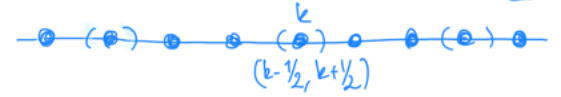
\includegraphics[scale=0.3]{images/def_subespacio_discreto} 
    \end{center}

    \item $a \in X, \mathcal{T}_a|_{X \setminus \{a\}} = $ discreta.
\end{enumerate}
\end{ej}

\begin{obs}
\begin{enumerate}
    \item $Y \subset_{\text{ab}} X: W \text{ abierto de } Y \Leftrightarrow W \text{ abierto de } X$ contenido en $Y$.
    \[
    \left[ W = U \cap Y^{\text{ab}},\ U^{\text{ab}} \subset X \Rightarrow W^{\text{ab}} \subset X \text{ por intersección finita} \right] 
    \]
    \item $Y \subset_{\text{cerr}} X: F \text{ cerrado de } Y \Leftrightarrow F \text{ cerrado de } X$ contenido en $Y$.
    \[
    \left[ C = F \cap Y^{\text{cerr}},\ F^{\text{cerr}} \subset X \Rightarrow C^{\text{cerr}} \subset X \text{ por intersección finita} \right] 
    \]
\end{enumerate}
\end{obs}

\chapter{Aplicaciones continuas}%
\label{cha:aplicaciones_continuas}
\section{Continuidad}%
\label{sec:continuidad}
El famoso $\varepsilon-\delta$ en $\mathbb{R}^n \mathcal{T}_u; x_0 \in X,\ f : \overbrace{X}^{\subset \mathbb{R}^p} \rightarrow \overbrace{Y}^{\subset \mathbb{R}^q}$: 
\begin{gather*}        
\forall \varepsilon > 0, \exists \delta > 0: 
\begin{cases}
    \lVert x - x_0 \rVert < \delta \Rightarrow \lVert f\left( x \right) - f\left( x_0 \right) \rVert < \varepsilon \Leftrightarrow\\
    x \in B\left( x_0, \delta \right) \Rightarrow f\left( x \right) \in B\left( f\left( x_0 \right), \varepsilon \right) \Leftrightarrow\\
    f\left( B\left( x_0, \delta \right) \right) \subset B\left( f\left( x_0 \right), \varepsilon \right) 
\end{cases} \Rightarrow\\
\boxed{\forall B\left( f\left( x_0 \right), \varepsilon \right),\ \exists B\left( x_0, \delta \right) \subset f^{-1}\left( B\left( f\left( x_0 \right), \varepsilon \right) \right)} 
.\end{gather*}

\begin{defi}
$f: X \rightarrow Y$ será \underline{continua en $x_0$} $\in X$ si: 
\[
\forall V^{f\left( x_0 \right)}: f^{-1}\left( V^{f\left( x_0 \right)} \right) = V^{x_0} 
\]
\end{defi}

\begin{prop}[Composición de continuidades]
La composición de funciones continuas es continua:

\[
X \xrightarrow{f} Y \xrightarrow{g} Z: \begin{rcases}
    f \text{ continua en } x_0\\
    g \text{ continua en } y_0
\end{rcases} \Rightarrow h = g \circ f \text{ continua en }  x_0
\]
\end{prop}
\begin{demo}
Sea $V^{h\left( x_0 \right)} \rightarrow h^{-1} V^{h\left( x_0 \right)} = f^{-1}g^{-1}V^{g\left( y_0 \right)} = f^{-1} V^{y_0} = V^{x_0}$.
\end{demo}

\begin{ej}
\begin{enumerate}
    \item $\forall f: X_{\text{discreta}} \rightarrow Y$ es continua. [Todo es abierto, luego todo es entorno en $\mathcal{T}_{\text{disc}}$]
    \item $\forall f: X \rightarrow Y_{\text{trivial}}$ continua. [$V^{f\left( x \right)} = Y$ es el único abierto, luego el único entorno, de $f^{-1}V^{f\left( x \right)} = f^{-1}Y = X$ es abierto]
    \item $f: X \rightarrow Y_{\text{discreta}}$ es continua $\Rightarrow f$ localmente creciente.
        [$\{f\left( x_0 \right)\} = V^{f\left( x_0 \right)}$ en $\mathcal{T}_{\text{discr}} \xRightarrow[f\text{ cont.}]{} f^{-1}f\left( x_0 \right) = V^{x_0}\; \land \;f \equiv f\left( x_0 \right)$]
    \item $f: X \rightarrow Y$ localmente constante $\Rightarrow$ continua.

    [$\forall x_0 \in X, \exists U^{x_0} : f \stackrel{U^{x_0}}{\equiv} f\left( x_0 \right) \Rightarrow \forall V^{f\left( x_0 \right)}: f^{-1}V^{f\left( x_0 \right)} \supset U^{x_0} \Rightarrow f^{-1}V^{f\left( x_0 \right)} = V^{x_0}$ es entorno de $x_0$]
\end{enumerate}
\end{ej}

\begin{prop}
Son equivalentes:
\begin{enumerate}
    \item $f$ es continua.
    \item $f^{-1}\left( \text{abierto}  \right) = \text{abierto} ,\ \forall \text{abierto} \in Y$.
    \item $f^{-1}\left( \text{cerrado} \right) = \text{cerrado},\ \forall $ cerrado de $Y$.
    \item $f^{-1}\left( \mathring{A} \right) \subset \inter\left( f^{-1}\left( A \right) \right),\ \forall A \subset Y$
    \item $f\left( \overline{A} \right) \subset \overline{f\left( A \right)},\ \forall A \subset X$
\end{enumerate}
\end{prop}
\begin{demo}
\begin{enumerate}
    \item $1 \Rightarrow 2)$
    \[
        W^{\text{ab}} \subset Y \Rightarrow W \text{ ent. de } f\left( x \right),\ \forall x \in f^{-1}W \Rightarrow f^{-1} W \text{ ent. de } \forall x \in f^{-1}W \Rightarrow f^{-1} W \subset X 
    \]
    \item $2 \Rightarrow 3)$
    \[
        C_{\text{cerr}} \subset Y \Rightarrow Y \setminus C \subset Y \Rightarrow^{2)} \underbrace{f^{-1}\left( Y\setminus C \right)}_{= X \setminus f^{-1}C} \subset X \Rightarrow f^{-1}C \stackrel{\text{cerr}}{\subset} X 
    \]
    \item $3 \Rightarrow 5)$

    \[
        \overline{f\left( A \right)} \stackrel{\text{cerr}}{\subset} Y \Rightarrow^{3)} \underbrace{f^{-1}\overline{f\left( A \right)}}_{\subset f^{-1}f\left( A \right) \supset A} \subset X \Rightarrow \overline{A} \subset f^{-1}\overline{f\left( A \right)} \Rightarrow f\left( \overline{A} \right) \subset \overline{f\left( A \right)} 
    \]
    \item $5 \Rightarrow 4)$
    \begin{gather*}
        Y \setminus \mathring{A}\Rightarrow \overline{Y\setminus A} \supset \overline{f\left( X \setminus f^{-1}A \right)} \stackrel{5)}{\supset} f\left( \overline{X \setminus f^{-1}\left( A \right)} \right) = f\left( X \setminus \inter\left( f^{-1}A \right) \right) \Rightarrow\\
        X \setminus \inter\left( f^{-1}A \right) \subset f^{-1}\left( Y\setminus \mathring{A} \right) = X \setminus f^{-1}\left( \mathring{A} \right)\Rightarrow f^{-1}\left( \mathring{A} \right) \subset \inter\left( f^{-1}A \right) 
    .\end{gather*}

    \item $4 \Rightarrow 1)$
    \begin{gather*}
        V^{f\left( x \right)} \Rightarrow f\left( x \right) \in \inter\left( V^{f\left( x \right)} \right) \Rightarrow x \in f^{-1}\left( \inter\left( V^{f\left( x \right)} \right) \right) \subset \inter\left( f^{-1}V^{f\left( x \right)} \right) \Rightarrow \\
        f^{-1}V^{f\left( x \right) } \text{ entorno de } x.
    \end{gather*}
\end{enumerate}
\end{demo}

\begin{obs}
\begin{enumerate}
    \item Los cuatros primeros enunciados tratan sobre ``imágenes inversas''. Por ejemplo, la segunda dice que $f^{-1}\mathcal{T}_Y \subset \mathcal{T}_X$.
    \item Pensando que un punto adherente es un ``punto límite'', $5$ nos dice que ``la imagen del límite es el límite de la imagen''.
    \item $Id: \left( X, \mathcal{T}_1 \right) \rightarrow \left( X, \mathcal{T}_2 \right)$ es continua $\Rightarrow \mathcal{T}_2 \subset \mathcal{T}_1$. [$Id^{-1}\mathcal{T}_1 = \mathcal{T}_2]$
\end{enumerate}
Y no mencionamos todos los ejemplos conocidos en espacios afines $\mathbb{R}^n$ con $\mathcal{T}_u$.
\end{obs}

\section{Continuidad y subespacios}%
\label{sec:continuidad_y_subespacios}
\begin{prop}
Sea $f: X \rightarrow Y$ continua y $Z \subset X$ subespacio $\Rightarrow f|_Z : Z \rightarrow Y$ es continua.
\end{prop}
\begin{demo}
Se aplica el criterio ``imagen inversa de abierto es abierto'' y la fórmula:
\[
\left( f|_Z \right)^{-1} \left( A \right) = Z \cap f^{-1}A,\ \forall A \subset Y
\]
\end{demo}

\underline{Criterios de continuidad por recubrimientos.} Sea $f: X \rightarrow Y$. 
\begin{itemize}
    \item \textbf{Por abiertos:} $\exists X = \bigcup_{i \in  I} U_i: \forall f|_{U_i} : U_i \rightarrow Y$ es continua. 

    \begin{demo}
    $W \subset Y \Rightarrow$
    \[
    \begin{cases}
        f^{-1}W = \bigcup_{i \in  I} U_i \cap f^{-1} W = \bigcup_{i \in  I} \left( f|_{U_i} \right)^{-1} W\\
        \left( f|_{U_i} \right)^{-1}W \subset U_i \subset X \Rightarrow \left( f|_{U_i} \right)^{-1} W \subset X
    \end{cases}\Rightarrow f^{-1}W \subset X  
    \]
    Por unión de abiertos.
    \end{demo}

    \item \textbf{Por cerrados:} $\exists X = \bigcup_{i = 0}^{n} F_i: \forall f|_{F_i} : F_i \rightarrow Y$ es continua. 

    \begin{demo}
    $C \subset Y \Rightarrow$
    \[
    \begin{cases}
        f^{-1}C = \bigcup_{i \in  I} F_i \cap f^{-1} C = \bigcup_{i \in  I} \left( f|_{F_i} \right)^{-1} C\\
        \left( f|_{F_i} \right)^{-1}C \subset F_i \subset X \Rightarrow \left( f|_{F_i} \right)^{-1} C \subset X
    \end{cases}\Rightarrow f^{-1}C \subset X  
    \]
    Por unión finita de cerrados.
    \end{demo}
\end{itemize}

\section{Homeomorfismos}%
\label{sec:homeomorfismos}
Recordemos las definiciones de continuidad que hemos visto:
\[
f \text{ continua} \Leftrightarrow f^{-1}\left( \text{abierto} \right) = \text{abierto} \Leftrightarrow f^{-1}\left( \text{cerrado} \right) = \text{cerrado} 
\]
Ahora veamos que ocurre al invertir la relación.
\begin{defi}
Sea $f: X \rightarrow Y$, será $\begin{cases}
    \text{\underline{abierta}} \\
    \text{\underline{cerrada}} 
\end{cases} \Leftrightarrow \begin{cases}
    f\left( \text{ab} \right) = \text{ab}\\
    f\left( \text{cerr} \right) = \text{cerr} 
\end{cases} $    
\end{defi}

%TODO: Fix observación
\begin{obs}
Cuidado: Continuidad no implica que sea abierta, cerrada ni viceversa.
\end{obs}

\begin{ej}
\begin{enumerate}
    \item $Id: X_{\text{trivial}} \rightarrow X_{\text{discreta}}$, -cont. +ab. +cerr.
    \item $Id: X_{\text{discreta}} \rightarrow X_{\text{trivial}}$, +cont. -ab. -cerr.
    \item $j: \left[ 0, 1 \right] \subset \mathbb{R}_{u}$, +cont. -ab. +cerr.
    \item $j: \left( 0, 1 \right) \subset \mathbb{R}_u$, +cont. +ab. -cerr.
\end{enumerate}
\end{ej}

\begin{prop}[Trivialidades esenciales]
Sea $f$ biyectiva, es equivalente:
\begin{itemize}
    \item $f$ es abierta
    \item $f$ es cerrada
    \item $f^{-1}$ es continua.
\end{itemize}
\end{prop}
\begin{demo}
\begin{enumerate}
    \item $F_{\text{cerr}} \subset X \Rightarrow X\setminus F_{\text{ab}} \subset X \Rightarrow^{ f\text{ ab}} \underbrace{f\left( X\setminus F \right)}_{= Y\setminus f\left( F \right) \text{(biy.)}} \subset_{\text{ab}} X \Rightarrow f\left( F \right) \subset_{\text{cerr}} Y \Rightarrow f$ cerr.

    \item $F_{cerr} \subset X \Rightarrow^{f \text{cerr}} \underbrace{f\left( F \right)}_{= \left( f^{-1} \right)^{-1} \left( F \right) \text{(biy)}} \subset_{\text{cerr}} Y \Rightarrow f^{-1}$ cont.

    \item $U_{\text{ab}} \subset X \Rightarrow^{f^{-1} \text{cont}} \underbrace{\left( f^{-1} \right) ^{-1} \left( U \right) }_{f\left( U \right) \text{(biy.)}} \subset Y \Rightarrow f$ ab.
\end{enumerate}
\end{demo}

\begin{defi}
    Sea $f: X \rightarrow Y$ biyectiva, es \underline{homeomorfismo} si $f\ \&\ f^{-1}$ son continuas, o equivalentemente si:
    \[
    \begin{cases}
        f \text{ biy.}\\
        \text{cont.}\\
        \text{ab.} 
    \end{cases} \Leftrightarrow \begin{cases}
        f \text{ biy.}\\
        \text{cont.}\\
        \text{cerr.}
    \end{cases} 
    \]
\end{defi}

\begin{defi}[Localización de un homeomorfismo]
Sea $f: X \rightarrow Y$, es \underline{homeomorfismo local} en $x_0 \in X$ si $f: V^{x_0} \rightarrow V^{f\left( x_0 \right)}$ es homeomorfismo para entornos de $x_0$ y $f\left( x_0 \right)$. Se suele decir para entornos ``suficientemente pequeños''.
\end{defi}

\underline{Ejercicio:} Se pueden tomar $V^{x_0}, V^{f\left( x_0 \right)}$ abiertos.

\begin{obs}
Un homeomorfismo local es abierto.
\end{obs}
\begin{demo}
    $U \subset_{\text{ab}} X \Rightarrow f\left( U \right)$ entorno $\forall y_0 = f\left(\overbrace{x_0}^{\in U}\right) \in f\left( U \right)$.
    Como $f$ homeomorfismo local $\Rightarrow f| : V^{x_0} \rightarrow V^{y_0}$ es homeomorfismo $\Rightarrow f\left( \overbrace{U \cap V^{x_0}}^{\ni y_0 = f\left( x_0 \right)} \right) \subset_{\text{ab}} V^{y_0} \Rightarrow f\left( \overbrace{U \cap V^{x_0}}^{\subset f\left( U \right)} \right)$ entorno de $y_0 \Rightarrow f\left( U \right)$ entorno de $y_0$.
\end{demo}

\begin{ej}[¡Importantes!]
\begin{enumerate}
    \item Proyección estéreo? $\mathbb{S}^{m} \setminus \{\text{punto}\} \rightarrow \mathbb{R}^m$ homeomorfismo.
    \item Proyección exponencial $\mathbb{R} \rightarrow \mathbb{S}': \theta \mapsto e^{2\pi i\theta} = \left( \cos 2\pi \theta, \sin 2\pi \theta \right)$, homeomorfismo local.
    \item Proyección antipodal: $\mathbb{S}^m \rightarrow \mathbb{R}P^{m}: x \mapsto \left[ x \right]$ homeomorfismo local.
    \item Lemniscata: $f: \mathbb{R} \rightarrow X \subset \mathbb{R}^2: t \mapsto \left( \frac{t}{1 + t^4}, \frac{t^3}{1 + t_4} \right)$ es biy. cont, pero \underline{no} homeomorfismo local.

    %TODO: Dibujo Lemniscata
    Engañosamente: 
    \[
        \forall t \in \mathbb{R} \exists \left( t - \varepsilon, t + \varepsilon \right) = I_{\varepsilon}: f| : I_{\varepsilon} \rightarrow f\left( I_{\varepsilon} \right) 
    \]
    es homeomorfismo.

    En $t = 0, f\left( I_{\varepsilon} \right)$ \underline{no} es entorno de $f\left( 0 \right) = \left( 0, 0 \right)$.
\end{enumerate} 
\end{ej}

\begin{defi}
Una \underline{variedad topológica} de $\dim m$ es un espacio localmente homeomorfo a $\mathbb{R}^m$, es decir, cada punto tiene un entorno abierto homeomorfo a una bola $B\left( 0, \varepsilon \right) \subset \mathbb{R}^m$ (luego a cualquier bola, luego a todo $\mathbb{R}^m$).
\end{defi}
\begin{ej}
Esferas, espacios proyectivos, toros...
\end{ej}

\chapter{Construcciones}%
\label{cha:construcciones}
\section{Imágenes inversas}%
\label{sec:imagenes_inversas}
\underline{Problema:} Hacer $f: Y \rightarrow \left( X, \mathcal{T} \right)$ continua con $\begin{cases}
    \text{top. discreta en } Y \text{ (matricialidad)}\\
    \text{top. \underline{menos fina} en } Y 
\end{cases}$ 

\underline{Sol:} $f^{-1} \mathcal{T} = \{f^{-1}U: U \in \mathcal{T}\}$ top. \underline{imagen inversa}. 
\begin{enumerate}
    \item Es topología (inm.)
    \item Es mínima. [$f$ es continua $\Rightarrow \forall f^{-1}U$ es abierto]
\end{enumerate}


%TODO: Fix teorema
\begin{theo}[Caracterización imagen inversa]
\begin{enumerate}
    \item
    \[
    \mathcal{T}' = f^{-1}\mathcal{T} \Leftrightarrow  
    \]
    \begin{equation}
        \forall g \left[ g \text{ cont.} \Leftrightarrow f \circ g \text{ cont.} \right]
    \end{equation}

    \item Y.
    %TODO: Fix composición
    \begin{center}
        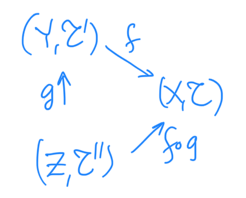
\includegraphics[scale=0.3]{images/caracterizacion_img_inv} 
    \end{center}
\end{enumerate}
\end{theo}
\begin{demo}
\begin{enumerate}
    \item $\mathcal{T}' = f^{-1}\mathcal{T}: $ 
    \begin{itemize}
        \item $g$ cont. $\Rightarrow f \circ g$ cont. (Composición de continuas)
        \item $f \circ g$ cont. $\Rightarrow g$ cont. ($V \in \mathcal{T}' \Rightarrow g^{-1}V \stackrel{\mathcal{T}' = f^{-1}\mathcal{T}}{=} g^{-1} f^{-1}U = \left( f \circ \right)^{-1} U \stackrel{f \circ g \text{ cont.}}{\in} \mathcal{T}''$)
    \end{itemize}

    \item Por otro lado,
    %TODO: Fix
    \begin{center}
        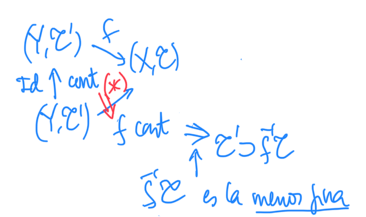
\includegraphics[scale=0.4]{images/dem_carac_img_inv_1} 
        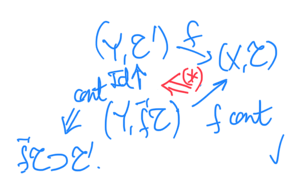
\includegraphics[scale=0.4]{images/dem_carac_img_inv_2} 
    \end{center}
\end{enumerate}
\end{demo}

\underline{Ejercicio}: Demostrar (ii) sin usar que $f^{-1}\mathcal{T}$ es la menos fina (usar que cumple la caracterización).

La anterior caracterización se llama \underline{propiedad universal}.

Caso esencial: 
\[
\boxed{f: Y \rightarrow X \text{ inyectiva}} 
\]

\begin{defi}
Una aplicación continua \underline{inyectiva} $f: \left( Y, \mathcal{T}' \right) \rightarrow \left( X, \mathcal{T} \right)$ tal que $\mathcal{T}' = f^{-1} \mathcal{T}$ se llama \underline{inmersión} (se suelen omitir las topologías).
\end{defi}

\begin{obs}
\begin{enumerate}
    \item $\mathcal{T}' = f^{-1}\mathcal{T} \Leftrightarrow \left( Y, \mathcal{T}' \right) \xrightarrow{\text{homeomorfismo}} \left( f\left( Y \right), \mathcal{T}|_{f\left( Y \right)} \right)$
    \[
    [V \in f^{-1}\mathcal{T} \Leftrightarrow V = f^{-1}\underbrace{U}_{\mathcal{T}} = f^{-1}\left( \underbrace{U \cap f\left( Y \right)}_{\mathcal{T}\mid f\left( Y \right)} \right)] 
    \]

    \item $f: Y \rightarrow X$ $1-1$ cont. $+ \begin{cases}
        \text{ab. } \Rightarrow \text{inmersión } [\text{ab. en } X \Rightarrow \text{ab. en } f\left( Y \right)\\
        \text{cerr.} \Rightarrow \text{inmersión } [\text{cerr. en } X \Rightarrow \text{cerr. en} f\left( Y \right)] 
    \end{cases} $
    \[
    \begin{cases}
        f\left( Y \right) \stackrel{\text{ab.}} X: V = f^{-1}U \in f^{-1}\mathcal{T} \Rightarrow fV = U \cap f\left( Y \right) \in \mathcal{T} \left( \text{inter. abierto} \right)\\
        f\left( Y \right) \stackrel{\text{cerr.}} X: C \text{ c.} f^{-1}\mathcal{T} \Rightarrow Y\setminus C = f^{-1} U \in f^{-1}\mathcal{T} \Rightarrow f\left( C \right) \left( X\setminus U \right) \cap f\left( Y \right) \stackrel{\text{cerr.}}{\subset} X \text{ i. c.} 
    \end{cases} 
    \]

    \item Tenemos: 
    \begin{itemize}
        \item Inmersión $ + \not$ ab. $+ \not$ cerr.
        \item Inmersión $+$ ab. $+ \not $ cerr.
        \item Inmersión $+$ ab. $+$ cerr.
    \end{itemize}
\end{enumerate}
\end{obs}

\begin{obs}
Las inmersiones permiten considerar unos espacios como subespacios de otros. Las frases ``el plano proyectivo real no es un subespacio de $\mathbb{R}^3$'', ``la esfera no es un subespacio de $\mathbb{R}^2$'', ``el plano proyectivo real es un subespacio de $\mathbb{R}^4$'' se refieren a esto: \underline{cuándo hay o no hay} una inmersión del primer espacio en el segundo, es decir, un subespacio del segundo homeomorfismo al primero. Es un problema fundamental de la topología
y de la geometría.
\end{obs}

\section{Imágenes directas}%
\label{sec:imagenes_directas}
\underline{Problema:} Hacer $f: \left( X, \mathcal{T} \right) \rightarrow Y$ continua en $\begin{cases}
    \text{top. trivial en } Y \text{(matrivialidad)}\\
    \text{top. \underline{más fina} en } Y 
\end{cases} $ 

\underline{Sol:} $f\mathcal{T} = \{V \subset Y: f^{-1}V \in \mathcal{T}\}$ top. \underline{imagen directa}.
\begin{enumerate}
    \item Es topología (inm.)
    \item Máxima [$f$ es continua $\Leftrightarrow \forall f^{-1} V$ es abierto] 
\end{enumerate}

\begin{theo}[Caracterización imágenes directas]
\begin{enumerate}
    \item
    \[
    \mathcal{T}' = f\mathcal{T} \Leftrightarrow  
    \]
    \begin{equation}
        \forall g \left[ g \text{ cont.} \Leftrightarrow g \circ f \text{ cont.} \right]
    \end{equation}

    \item Y.
    %TODO: Fix composición
    \begin{center}
        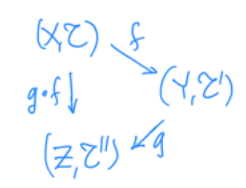
\includegraphics[scale=0.3]{images/caracterizacion_img_dir} 
    \end{center}
\end{enumerate}
\end{theo}
\begin{demo}
\begin{enumerate}
    \item $\mathcal{T}' = f^{-1}\mathcal{T}: $ 
    \begin{itemize}
        \item $g$ cont. $\Rightarrow g \circ f$ cont. (Composición de continuas)
        \item $g \circ f$ cont. $\Rightarrow g$ cont. ($W \in \mathcal{T}'' \Rightarrow f^{-1}\left( g^{-1} W \right) = \underbrace{\left( g \circ f \right)}_{\text{cont.}}^{-1} W \in \mathcal{T} \stackrel{\mathcal{T}' = f\mathcal{T}}{\Rightarrow} g^{-1}W \in \mathcal{T}'$)
    \end{itemize}

    \item Por otro lado,
    %TODO: Fix
    \begin{center}
        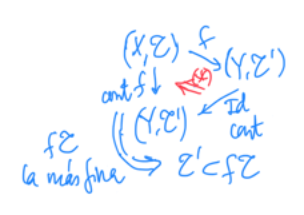
\includegraphics[scale=0.4]{images/dem_carac_img_dir_1} 
        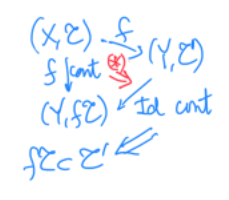
\includegraphics[scale=0.4]{images/dem_carac_img_dir_2} 
    \end{center}
\end{enumerate}
\end{demo}

\underline{Ejercicio}: Demostrar (ii) sin usar que $f\mathcal{T}$ es la más fina (usar que cumple la caracterización)

La caracterización anterior se llama \underline{propiedad universal}.

\begin{obs}
$f\left( X \right)$ es abierto y cerrado en $f\mathcal{T}: \begin{cases}
    \forall y \in Y \setminus f\left( X \right), f^{-1}y = \emptyset \in \mathcal{T} \Rightarrow \{y\} \in f\mathcal{T}\\
    f^{-1}f\left( X \right) = X \in \mathcal{T} \Rightarrow f\left( X \right) \in f\mathcal{T}
\end{cases}$
\end{obs}

Caso esencial:
\[
\boxed{f: X \rightarrow Y \text{ sobreyectiva}.} 
\]
Para entender los abiertos de una imagen directa es conveniente representarlos en el dominio. El concepto es conjuntista en realidad:

\begin{defi}
Un conjunto $A \subset X$ es \underline{saturado} (respecto de $f$) si $f^{-1}f\left( A \right) = A$.
\end{defi}
\begin{prop}
Los abiertos de $f\mathcal{T}$ son las imágenes de los abiertos saturados de $\mathcal{T}$.    
\end{prop}
\begin{demo}
\begin{enumerate}
    \item $V \in f\mathcal{T} \Rightarrow f^{-1}V \in \mathcal{T}$ y $V \stackrel{f \text{ sobre}}{=} f^{-1}fV$
    \item $U \in \mathcal{T}$, saturado $\Rightarrow f\left( U \right) = V \in f\mathcal{T}: f^{-1}V = f^{-1}f\left( U \right) \stackrel{U \text{ sat.}}{=} U \in \mathcal{T}$
\end{enumerate}
\end{demo}

\begin{obs}
Los abiertos \underline{no} saturados de $X$ pueden tener imágenes \underline{no} abiertas de $Y$. 
\end{obs}

\begin{ej}
\begin{enumerate}
    \item $f: \left[ 0, 1 \right] \rightarrow \mathbb{S}^1 = Y: t \mapsto \left( \cos 2\pi t, \sin 2\pi t \right) = \exp\left( 2 \pi i t \right)$
    %TODO: Fix image
    \begin{center}
        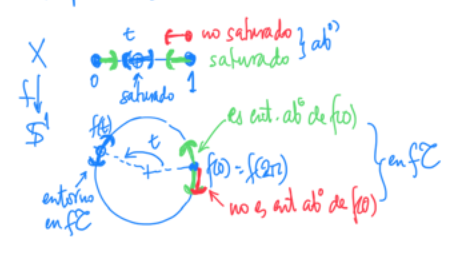
\includegraphics[scale=0.4]{images/ej_sat_1} 

        \textit{La topología imagen directa es la usual en $\mathbb{S}^1$.} 
    \end{center}

    \item Tenemos:
    \begin{align*}
        f: R = \left[ 0, 1 \right] \times \left[ 0, 1 \right] &\rightarrow C \subset \mathbb{R}^3: x^2 + y^2 = 1,\ 0 \le z \le 1\\
        \left( s, t \right) &\mapsto \left( \cos 2\pi s, \sin 2\pi s, t \right) 
    .\end{align*}

    %TODO: Fix image
    \begin{center}
        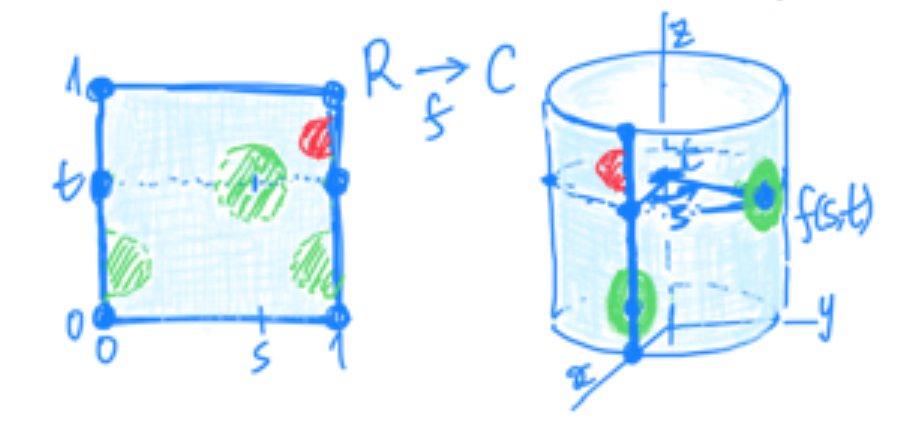
\includegraphics[scale=0.3]{images/ej_top_dir_2}

        \textit{Analizando los abiertos saturados y no saturados se concluye que la topología imagen directa es la usual en el tronco del cilindro.} 
    \end{center}
\end{enumerate}
\end{ej}

\begin{defi}
Una aplicación continua sobre $f: \left( X, \mathcal{T} \right) \rightarrow \left( Y, \mathcal{T}' \right)$ tal que $\mathcal{T}' = f\mathcal{T}$ se llama \underline{identificación} (se suelen omitir las topologías)
\end{defi}

\begin{obs}
\begin{enumerate}
    \item Identificación: $V \stackrel{\text{ab}}{\subset} Y \Leftrightarrow f^{-1}V \stackrel{\text{ab}}{\subset} X$

    Continua: $V \stackrel{\text{ab}}{\subset } Y \Rightarrow f^{-1}V \stackrel{\text{ab}}{\subset} X$

    \item Sea $f: X \rightarrow Y$ sobre. continua. Si además es:
    \begin{itemize}
        \item Abierta $\Rightarrow f$ es identificación [por (1)]
        \item Cerrada $\Rightarrow f$ es identificación [$f^{-1}V \stackrel{\text{ab}}{\subset} X \stackrel{\text{+ cerr.}}{\Rightarrow} f\left( \underbrace{X \setminus f^{-1}\left( V \right)}_{= Y\setminus V} \right) \stackrel{\text{cerr.}}{\subset} Y \Rightarrow V \stackrel{\text{ab}}{\subset} Y$
    \end{itemize}
\end{enumerate}
\end{obs}

\begin{defi}[Cociente]
Dentro de las identificaciones tenemos un caso particular: $\left( X, \mathcal{T} \right) \stackrel{p}{\rightarrow} Y = \underbrace{X / \sim}_{p \mathcal{T} = \text{top. cociente}}$. Cociente respecto de una relación de equivalencia en $X$. 
\end{defi}
%TODO: Fix imagen
\begin{center}
    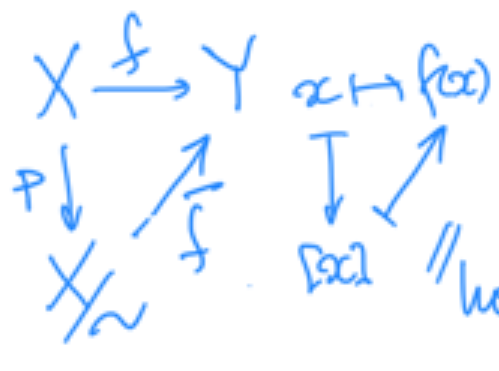
\includegraphics[scale=0.2]{images/def_cociente} 
\end{center}
Tenemos que $x_1 \sim x_2 \stackrel{\text{def}}{\Leftrightarrow} f\left( x_1 \right) = f\left( x_2 \right)$. Homeoforma de $p\mathcal{T}$ sobre $f\mathcal{T} \Leftrightarrow f$ identificación tal que:
\[
\begin{cases}
    \overline{f} \text{ es biyección}\\
    p^{-1}V = f^{-1}\overline{f} V \text{ y } f^{-1}W = p^{-1} \overline{f}^{-1}W
\end{cases} 
\]

\begin{pg}
    Los cocientes son cómodos para definir espacios, las identificaciones son mejores para estudiar las propiedades que tenemos. Conviene pues tener triángulos como el anterior. Se puede contemplar $Y$ como un modelo del cociente.
\end{pg}

%TODO: Fix imágenes
\begin{ej}[Anteriores]
La circunferencia y el cilindro como cocientes:
\begin{center}
    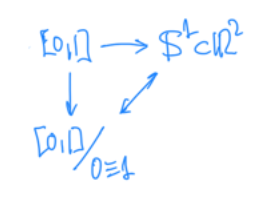
\includegraphics[scale=0.4]{images/ej_cociente_1} 
    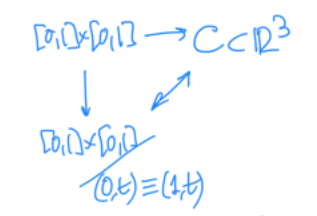
\includegraphics[scale=0.4]{images/ej_cociente_2}
\end{center}

Para representar cocientes se utilizan dibujos que indican las identificaciones en los espacios de partida:
%TODO: Fix
\begin{center}
    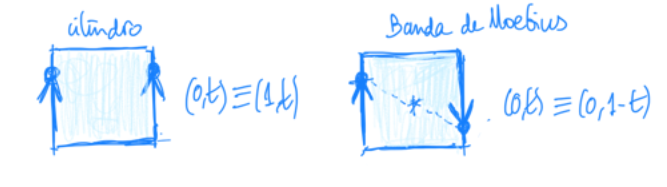
\includegraphics[scale=0.3]{images/ej_cociente_3} 
\end{center}
\end{ej}

\section{Productos (finitos)}%
\label{sec:productos_finitos_}
\underline{Problema:} Hacer $X_1 \times \ldots \times X_r = Y \xrightarrow{p_i} \left( X_i, \mathcal{T}_i \right), 1 \le i \le r$ continuas con 
\[
\begin{cases}
    \text{top. discreta en } Y \text{ matrivialidad}\\
    \text{top. \underline{menos fina} en} Y
\end{cases} 
\]
\underline{Solución:} $p_i$ cont. $\Rightarrow p_i^{-1} \underbrace{U_i}_{\mathcal{T}_i} = \underbrace{X_1 \times \ldots \times U_i \times \ldots \times X_r}_{\text{deben ser abiertos}}  \Rightarrow \bigcap_{i} p_i^{-1}U_i = \underbrace{U_1 \times \ldots \times U_r}_{\text{abiertos}}$ pero \underline{no} son topología $\Rightarrow$
\[
\mathcal{B} = \{U_1 \times \ldots \times U_r: U_i \in \mathcal{T}_i \} \text{ es la \underline{base} de la \underline{topología producto}: } \boxed{\prod_{i} \mathcal{T}_i} 
\]
\begin{ej}
La $\mathcal{T}_u$ en $\mathbb{R}^n$ ese el producto de la usual en cada factor $\mathbb{R}$ de $\mathbb{R}^n$. La base de la definición de topología producto está formada por las ``bolas cuadradas''.
\end{ej}

%TODO: Fix teorema
\begin{theo}[Caracterización topología producto]
\begin{enumerate}
    \item
    \[
    \mathcal{T}' = \prod_{i} \mathcal{T} \Leftrightarrow  
    \]
    \begin{equation}
        \forall g \left[ g \text{ cont.} \Leftrightarrow \forall g_i \text{ cont.} \right]
    \end{equation}

    \item Y.
    %TODO: Fix composición
    \begin{center}
        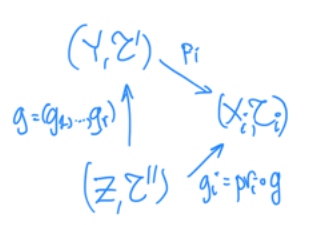
\includegraphics[scale=0.3]{images/caracterizacion_top_prod} 
    \end{center}
\end{enumerate}
\end{theo}
\begin{demo}
\begin{enumerate}
    \item $\mathcal{T}' = \prod_{i} \mathcal{T}: $ 
    \begin{itemize}
        \item $g$ cont. $\Rightarrow g_i$ cont. (Composición de continuas)
        \item $g_i$ cont. $\Rightarrow g^{-1}\left( U_1 \times \ldots \times U_r \right) = \underbrace{g_1^{-1}\left( U_1 \right)}_{\mathcal{T}''} \cap \ldots \cap \underbrace{g_r^{-1}\left( U_i \right)}_{\mathcal{T}''} \in \mathcal{T}''$ (intersección finita de abiertos) 
    \end{itemize}

    \item Por otro lado,
    %TODO: Fix
    \begin{center}
        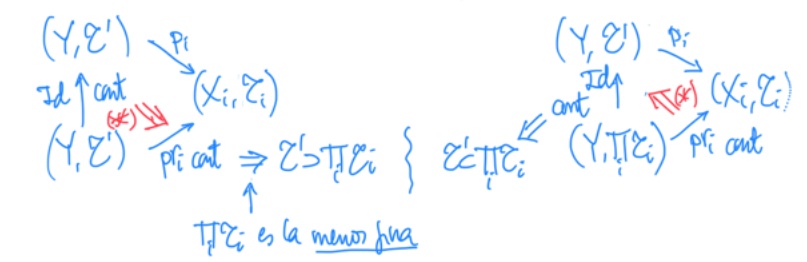
\includegraphics[scale=0.4]{images/dem_carac_top_prod} 
    \end{center}
\end{enumerate}
\end{demo}

\begin{ej}
Demostrar (ii) sin usar que $\prod_{i} \mathcal{T}_i$ es la menos fina (usar que cumple la caracterización)
\end{ej}

La anterior caracterización se llama \underline{propiedad universal}.

\begin{prop}
\begin{enumerate}
    \item $p_i: Y \rightarrow X_i$ es abierta. [$p_i\left( U_1 \times \ldots \times U_r \right) = U_i$]
    \item $X_j \xrightarrow{\alpha_j} Y: x_j \mapsto \left( a_1, \ldots, x_j, \ldots, a_r \right)$ es inmersión ($a_i \in X_i$ fijados).
    \[
    \left[\begin{cases}
        \alpha_j\left( X_j \right) = \{a_1\} \times \ldots \times X_j \times \ldots \times \{a_r\} \\
        \alpha_j\left( U_j \right) = \{a_1\} \times \ldots \times U_j \times \ldots \times \{a_r\} = \alpha\left( X_j \right) \cap \left( X_1 \times \ldots \times U_j \times \ldots \times X_r \right) 
    \end{cases}\right]     
    \]
\end{enumerate}
\end{prop}

\begin{pg}
En una topología producto ``todo se genera en productos''.
\begin{ej}
\begin{itemize}
    \item Bases de entornos: $\mathcal{V}^a = \mathcal{V}^{a_1} \times \ldots \times \mathcal{V}^{a_r} \stackrel{mut??}{=} \{V_1 \times \ldots \times V_r: V_i \in \mathcal{V}^{a_i}\} \left( a \in Y \right)$.
    \item Base de abiertos: $\mathcal{B} = \mathcal{B}_1 \times \ldots \times \mathcal{B}_r = \{B_1 \times \ldots \times B_r: B_i \in \mathcal{B}_i\}$ (esto repite la construcción de $\prod_{i} \mathcal{T}_i$)
\end{itemize}
\end{ej}
\end{pg}

\section{Sumas (finitas)}%
\label{sec:sumas_finitas_}
\underline{Problema:} Hacer $\left( X_i, \mathcal{T}_i \right) \xrightarrow{e_i} Y = X_1 + \ldots X_r = \left( X_1 \times \{1\} \right) \cup \ldots \cup \left( X_r \times \{r\} \right), 1 \le i \le r: x_i \mapsto \left( x_i, i \right)$ continuas, ,con 
\[
\begin{cases}
    \text{top. trivial en } Y \text{ matrivialidad}\\
    \text{top. \underline{más fina} en} Y
\end{cases} 
\]
\underline{Solución:} $\underbrace{U_i}_{\mathcal{T}_i} \in e_i^{-1}\left( U_i \times \{i\} \right) \Rightarrow \mathcal{B} = \{U_1 \times \{1\}, \ldots, U_r \times \{r\}: U_1 \in \mathcal{T}_1, U_r \in \mathcal{T}_r\}$ es base de una topología en $Y$, la topología \underline{suma}: $\mathcal{T}_1 + \ldots + \mathcal{T}_r$.

\begin{prop}
$\forall i, e_i: \left( X_i, \mathcal{T}_i \right) \rightarrow \left( X_i\times \{i\}, \mathcal{T}|_{X_i \times \{i\}} \right)$ es inmersión abierta y cerrada.
\end{prop}
\begin{demo}
\begin{itemize}
    \item Inmersión abierta: $e_i\left( U_i \right) = U_i \times \{i\} \in \mathcal{T}$
    \item Cerrada: $Y\setminus e_i\left( X_i \right) = Y \setminus X_i \times \{i\} = \bigcup_{j \neq i} X_j \times \{j\} \in \mathcal{T}$
\end{itemize}
\end{demo}

%TODO: Fix teorema
\begin{theo}[Caracterización topología suma]
\begin{enumerate}
    \item
    \[
    \mathcal{T}' = \mathcal{T}_1 + \ldots + \mathcal{T}_r \Leftrightarrow  
    \]
    \begin{equation}
        \forall g \left[ g \text{ cont.} \Leftrightarrow \forall g_i \text{ cont.} \right] \text{(Propiedad universal)} 
    \end{equation}

    \item Y.
    %TODO: Fix composición
    \begin{center}
        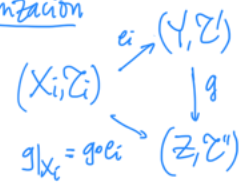
\includegraphics[scale=0.3]{images/caracterizacion_top_sum} 
    \end{center}
\end{enumerate}
\end{theo}
%TODO: Tal vez hacerlo bien?
\begin{demo}
    Análoga a las anteriores construcciones.
\end{demo}

\begin{pg}
Localmente $Y = X_1 + \ldots + X_r$ es como sea cada $X_i$. Por ejemplo, las bases de entornos de $Y$ son las de los sumandos. Globalmente, se trata cada sumando separadamente. Por ejemplo, las bases de abiertos de los sumandos se unen para dar una base de abiertos de $Y$. Olvidando el tecnicismo $X_i \times \{i\} \equiv X_i$:
\begin{center}
   $Y$ es unión disjunta de los sumandos\\
   Los sumando son subespacios abiertos y cerrados de $Y$
\end{center}
Es un formalismo para hacer cómodamente otras construcciones. Por ejemplo, ``pegar dos discos por sus bordes'' sería:
\begin{gather*}
    \text{disco} D \subset \mathbb{R}^2: x^2 + y^2 \le 1, \text{ borde } \partial D = \mathbb{S}^1: x^2 + y^2 = 1\\
    %TODO: Fix cociente
    D_1 + D_2 / \sim\quad \overbrace{\left( p, 1 \right)}^{\partial D} \sim \left( p, 2 \right) 
.\end{gather*}
%TODO Fix
\begin{center}    
    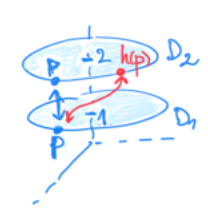
\includegraphics[scale=0.3]{images/pg_top_sum} 
\end{center}
y más elaborado $h: \partial D \stackrel{\text{homeo.}}{\approx} \partial D$ con $\overbrace{p}^{\in \partial D} \sim h\left( p \right)$.

Finalmente, hay otros conceptos de ``suma'' más significativos que veremos en algún ejemplo.
\end{pg}

\section{Espacios proyectivos reales}%
\label{sec:espacios_proyectivos_reales}
Como vimos en geometría lineal tenemos que: 
\[
\mathbb{R}P^n = \mathbb{P}^{n} = \mathbb{R}^{nH}\setminus \{0\} / \underbrace{\sim }_{\text{Prop.}} \Rightarrow \mathbb{P}^{n} = \{\text{rectas vectoriales de } \mathbb{R}^{n+1}\}     
\]
Que en coordenadas es:
\begin{align*}
    \pi: \mathbb{R}^{nH} \setminus \{0\} &\rightarrow \mathbb{P}^{n}\\
    \left( x_0, \ldots, x_n \right) &\mapsto \left( x_0 : \ldots : x_n \right) 
.\end{align*}
Las ecuaciones serán de la forma: $h\in \mathbb{R}\left[ x_0, \ldots, x_n \right]$ homogénea $\Rightarrow \begin{cases}
    h\left( x \right) = 0\\
    h\left( x \right) \neq 0
\end{cases}$ está bien definido en $\mathbb{P}^{n}$.
\[
\begin{rcases}
    %TODO: Fix lista
   \text{· Variedades proyectivas lineales}\\  
   \text{· Variedades proyectivas}\\
   \text{· Variedades proyectivas algebraicas}  
\end{rcases} \text{ecuaciones homogéneas de grado:} 
\begin{cases}
    1\\
    2\\
    \text{arbitrario} 
\end{cases} 
\]
\underline{Cartas afines:} 
\begin{gather*}
    \underbrace{H \subset \mathbb{P}^{n}}_{\text{hiperplano proyectivo}} \rightarrow \underbrace{\hat{H} \subset \mathbb{R}^{n + 1}}_{\text{hiperplano lineal} } : \underbrace{h = 0}_{\text{forma lineal}}, H = \hat{H} \setminus \{0\} / \sim  \\
    \pi|: \underbrace{\{h = 1\} \subset \mathbb{R}^{n + 1} \setminus \{0\}}_{\text{hiperplano afín}} \rightarrow \underbrace{\mathbb{P}^{n} \setminus H}_{\{h \neq 0\}} = 0 \text{ es biyección.}    
.\end{gather*}
Terminología: $H$ es \underline{hiperplano del infinito} de la \underline{carta afín} $U$.

Topología en $U$: La imagen directa de la usual en $\{h = 1\} \subset \mathbb{R}^{n + 1} \Rightarrow \pi|: \{h = 1\} \rightarrow U$ \underline{homeomorfismo}. 

%TODO: Fix subrayado
\underline{Topología en }$\mathbb{P}^{n}$: 
\begin{itemize}
    \item \underline{Cociente} de la usual vía $\mathbb{R}^{n+1}\setminus \{0\} \xrightarrow{\pi} \mathbb{P}^{n}: \left( x_0, \ldots, x_n \right) \mapsto \left( x_0 : \ldots : x_n \right)$
    \item ``\underline{Suma}'' de las definidas en las cartas afines:
    \[
        W \text{ abierto si } W \cap U \text{ es abierto } \forall U \text{ carta afín. [Es top. en } \mathbb{P}^{n}] 
    \]
\end{itemize}
Estas dos topologías coinciden.
\begin{demo}
\begin{enumerate}
    \item $U$ es abierto en la top. cociente. [$\pi^{-1} U = \{h \neq 0\}$ abierto usual]
    \item La topología cociente en $U$ coincide con la topología de carta afín:
    %TODO: Fix diagrama
    \begin{center}
        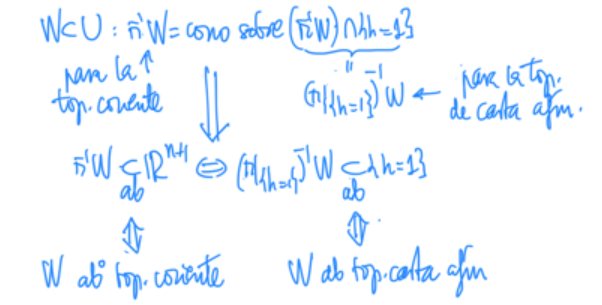
\includegraphics[scale=0.3]{images/eq_top_proyectivo} 
    \end{center}
    \item[1. + 2.] $\Rightarrow $ La top. cociente está generada por las topologías de las cartas afines, que forman un recubrimiento abierto de $\mathbb{P}^{n}$.
\end{enumerate}
\end{demo}

\begin{obs}
De lo anterior deducimos:
\begin{enumerate}
    \item $U_1, U_2$ dos cartas afines $\Rightarrow U_1 \cap U_2$ abiertos.
    \[
    \left[ \text{Cartas afines: } U_i = \{h_1 \neq 0\} \begin{cases}
        \pi|: \{h_1 = 1\} \rightarrow U_1 \text{homeo.}\\
        \left( \pi_1 \right)^{-1}\left( U_1 \cap U_2 \right) = \{h_1 = 1, h_2 \neq 0\} \stackrel{\text{ab.}}{\subset} \{h_1 = 1\}  
    \end{cases} \right] 
    \]
    \item Las topologías de $U_1$ y $U_2$ coinciden en $U_1 \cap U_2$.

    [De nuevo conviene entenderlo con cartas:
    %TODO: Fix
    \begin{center}
        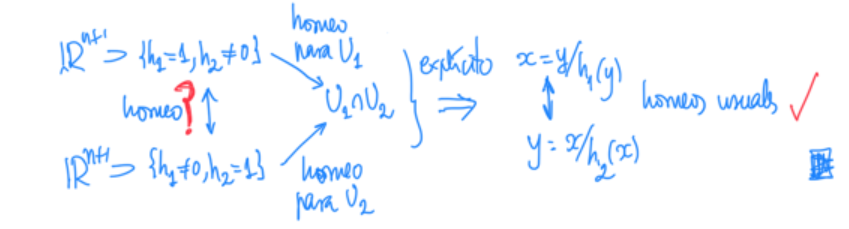
\includegraphics[scale=0.3]{images/obs_cartas_afines} ]
    \end{center}
\end{enumerate}
\end{obs}

%TODO: Esto es posible que se pueda agrupar mejor (hasta Möbius)
\underline{Atlas afín canónico}: No se suelen utilizar todas las cartas afines: $n + 1$ distintas ya cubren $\mathbb{P}^{n}$. Típicamente $\mathbb{P}^{n} = U_0 \cup \ldots \cup U_n$ con:
\[
U_i = \{x_i \neq 0\} \leftrightarrow \{\underbrace{x_i = 1}_{\equiv \mathbb{R}^n}\}: \left( x_0 : \ldots : x_i : \ldots : x_n \right) \mapsto \left( \frac{x_0}{x_i}, \ldots, \overbrace{1}^{\mathbb{R}^n \rightarrow}, \ldots, \frac{x_n}{x_i} \right), 0 \le i \le n
\]

\underline{Cociente antipodal}: Toda recta de $\mathbb{R}^{n + 1}$ corta a $\mathbb{S}^{n}: x_0^2 + \ldots + x_n^2 = 1$ en dos puntos \underline{antipodales}, así que denotamos un ``sub'' cociente, que es también identificación.
%TODO: Fix imagen
\begin{center}
    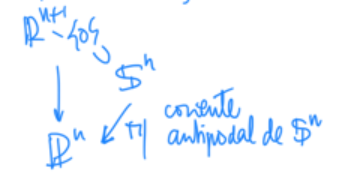
\includegraphics[scale=0.3]{images/cociente_antipodal} 

    [Como antes tenemos conos: $\pi^{-1}W = $ cono sobre $\underbrace{\mathbb{S}^n \cap \pi^{-1}W}_{= \left( \pi / \mathbb{S}^n \right)^{-1} W}$]
\end{center}

Las cartas afines tienen una representación muy conveniente:
%TODO: Fix imagen
\begin{center}
    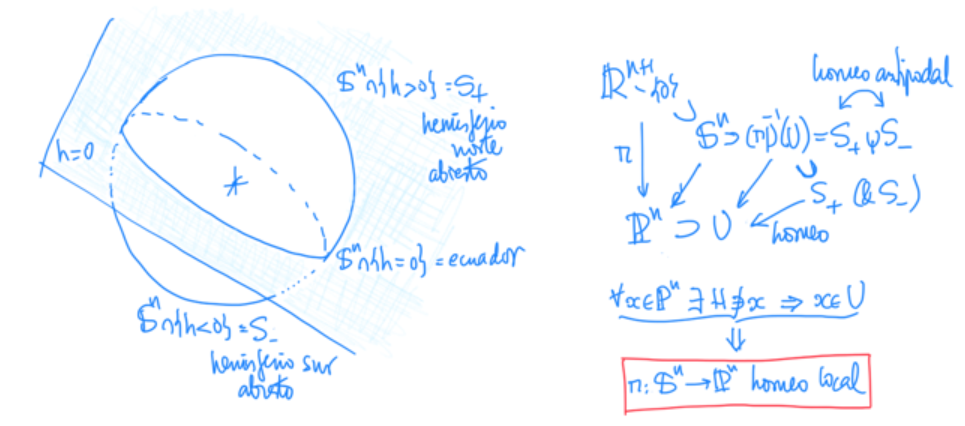
\includegraphics[scale=0.3]{images/repr_carta_afin} 
\end{center}

\underline{Cociente de un disco}:
\[
E = \{h = 0, x_0^2 + \cdots + x_n^2 = 1\} = \partial \begin{cases}
    \overline{S}_+ = \mathbb{S}^n \cap \{h \ge 0\} \text{ hemisferio cerrado.} \\
    D^n = \{h = 0, x_0^2 + \cdots + x_n^2 \le 1\} \text{ disco.} 
\end{cases} 
\]
%TODO: Fix imagen
\begin{center}
    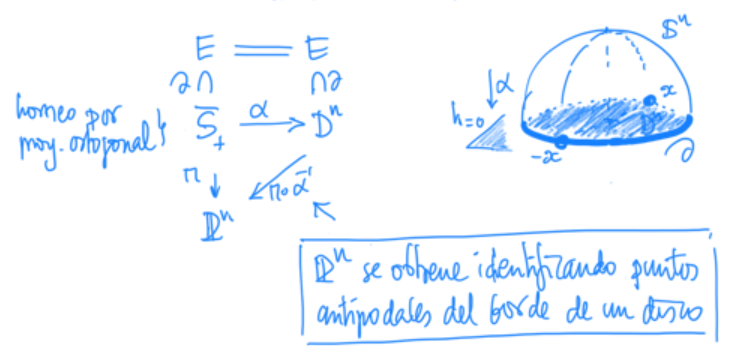
\includegraphics[scale=0.3]{images/cociente_disco} 
\end{center}

\begin{ej}
$\mathbb{P}^{2} \setminus D^2 = $ banda de Möbius.
%TODO: Fix imagen
\begin{center}
    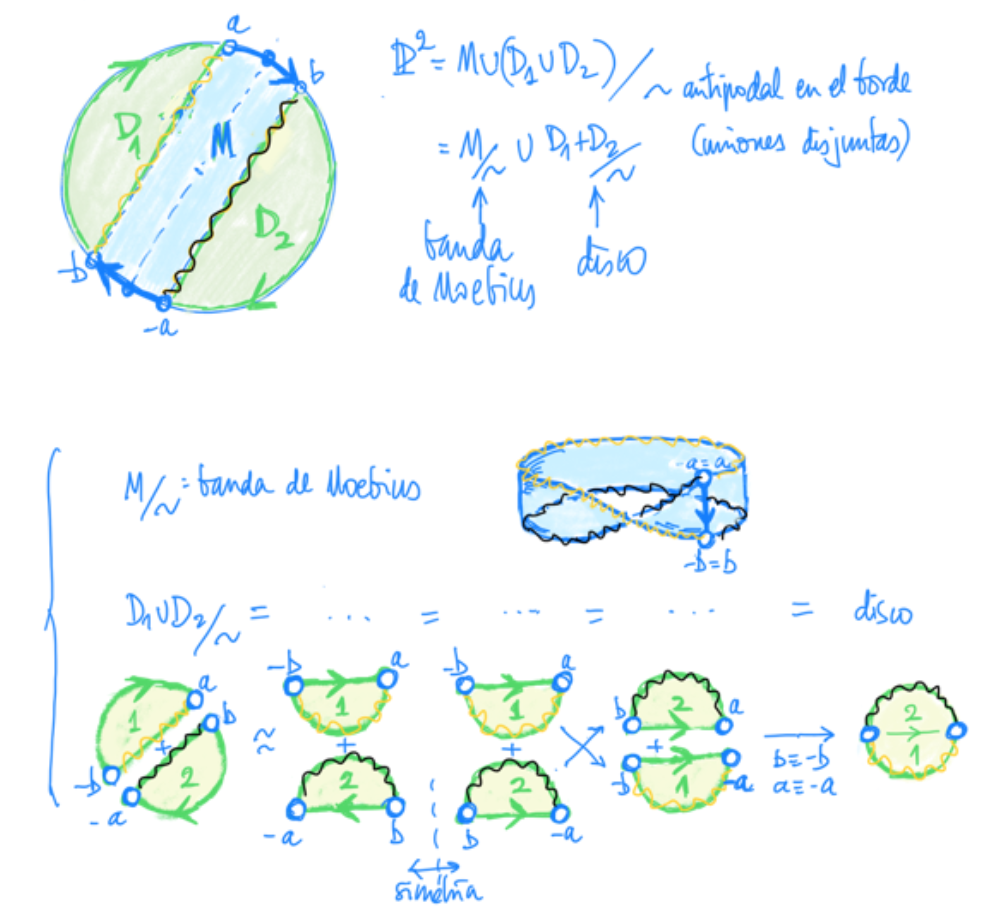
\includegraphics[scale=0.3]{images/banda_moebius} 
\end{center}
\end{ej}


\chapter{Separación}%
\label{cha:separacion}

\section{Concepto}%
\label{sec:concepto}
\begin{defi}
Un espacio $X$ es \underline{Hausdorff} o $T_2$ si cada par de puntos distintos $x, y \in X$ tienen entornos disjuntos: $V^x \cap V^y = \emptyset$. 
\end{defi}
Hay otras formas de separación, más débiles o más fuertes, pero nos contentaremos con ésta al ser la más intuitiva.
\begin{obs}
\begin{enumerate}
    \item Si existen entornos disjuntos, existen entornos abiertos disjuntos [$\forall V \supset U$]
    \item Si $X$ es Hausdorff, los puntos son cerrados.
    \[
    \left[ \forall y \neq x, \exists U^y \not\ni x \Rightarrow X \setminus \{x\} = \bigcup_{y \neq x} U^y  \text{ es abierto.} \right] 
    \]
    \item $\left( X, \mathcal{T}_{CF} \right)$ no es Hausdorff: dos abiertos cualesquiera se cortan ($X$ infinito) tiene puntos cerrados: $X\setminus \{x\}$ es abierto.

    \item $\left( \mathbb{R}^n, \mathcal{T}_{u} \right)$ es Hausdorff: $x \neq y \Rightarrow B\left( x, \varepsilon \right) \cap B\left( y, \varepsilon \right) = \emptyset$ si $\varepsilon \le \lVert x - y \rVert / 2$

    \item En $\left( X, \mathcal{T}_a \right)$ el punto $a$ no es cerrado: $a \not\in X \setminus \{a\} \Rightarrow X \setminus \{a\}$ no es abierto. $\forall x \neq a \forall U^x \supset \{a, x\} \ni a$ !!!.
\end{enumerate}
\end{obs}

\begin{prop}
Sean $f, g: X \rightarrow Y$ continuas con $Y$ Hausdorff $\Rightarrow \{f = g\} = \{x \in X : f\left( x \right) = g\left( x \right)\}$ es cerrado.
\end{prop}
\begin{demo}
\begin{enumerate}
    \item $f\left( x \right) \neq g\left( x \right) \xRightarrow{T_2} \exists V^{f\left( x \right) \cap V\left( g\left( x \right) \right)} = \emptyset \xRightarrow{\text{cont.}} f^{-1}V^{f\left( x \right)} \cap g^{-1}V^{g\left( x \right)} = V^x$ entorno de $x$.

    \item $V^x \cap \{f = g\} = \emptyset: y \in V^x \Rightarrow \begin{cases}
        f\left( y \right) \in V^{f\left( x \right)} \\
        g\left( y \right) \in V^{g\left( x \right)} 
    \end{cases} \Rightarrow f\left( y \right) \neq g\left( y \right)$

    \item[1. + 2.] $X\setminus \{f = g\} = \{f \neq g\}$ es entorno de todos sus puntos, luego abierto, luego $\{f = g\}$ es cerrado.
\end{enumerate}
\end{demo}

\begin{coro}
Si $f = g$ es un subconjunto denso, entonces $f \equiv g$
\end{coro}
\begin{demo}
$\exists \overline{A} = X: f|_A = g|_A \Rightarrow \{f = g\} \supset A \xRightarrow{\text{prop.}} \{f = g\} \supset \overline{A} = X$.
\end{demo}

\underline{Caso particular importante}:
Funciones $f: X \rightarrow \mathbb{R}$.

\begin{obs}
$f: X \rightarrow \underbrace{Y}_{\in T_2}$ continua $\Rightarrow f^{-1}\left( Y \right)$ cerrado $\forall y \in Y$.

Porque  los puntos de $Y$ son cerrados y, de hecho, eso basta.
\end{obs}

\section{Tabla de comportamiento}%
\label{sec:tabla_de_comportamiento}
Se trata de saber si la propiedad se conserva por las construcciones conocidas.

Se tiene:
\begin{center}
\begin{tabular}{ c | c | c | c | c |}
    & Subespacios & Cocientes & Productos & Sumas\\
    \hline
    $T_2$ & \checkmark & $\times$ & \checkmark & \checkmark\\
    \hline
\end{tabular}
\end{center}
\begin{enumerate}
    \item $Y \subset X = T_2: y_1, y_2 \in Y \Rightarrow \exists \underbrace{V^{y_1}}_{\text{En } X}  \cap V^{y_2} = \emptyset \Rightarrow \underbrace{\left( V^{y_1} \cap Y \right)}_{\text{En } Y}  \cap \left( V^{y_2} \cap Y \right) = \emptyset$.

    \item $Y = \mathbb{R}/\mathbb{Q}: \begin{rcases}
        y_1 = \mathbb{Q} \in Y\\
        y_2 = \sqrt{2} \in Y
    \end{rcases} \nexists V^{y_1} \cap V^{y_2} = \emptyset: $ todo entorno abierto de $\sqrt{2}$ contiene racionales, luego al saturar, contiene $\mathbb{Q}$.

    \item $X$ y $Y$ ambos $T_2 \Leftrightarrow X \times Y$ $T_2$.

        $\Rightarrow)$
        \[
        \left( x_1, y_1 \right) \neq \left( x_2, y_2 \right) \in X \times Y \Rightarrow \begin{cases}
            x_1 \neq x_2 \Rightarrow \exists V^{x_1} \cap V^{x_2} = \emptyset \Rightarrow \left( V^{x_1} \times Y \right) \cap \left( V^{x_2} \times Y \right) = \emptyset
        \end{cases}  
        \]

        $\Leftarrow)$
        \[
        X \approx X \times \{y_0\} \subset X \times Y, T_2 \xRightarrow{1} X\times \{y_0\} T_2 \Rightarrow XT_2
        \]
        %TODO: Image
        \begin{center}
            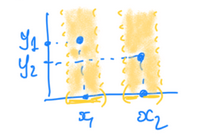
\includegraphics[scale=0.4]{images/t2_top_prod} 
        \end{center}

    \item $X$ y $Y$ ambos $T_2 \Leftrightarrow X + Y\ T_2$

    Único comentario: $x \in X$ y $y \in Y \Rightarrow X = V^x, Y = V^y$ y $X \cap Y = \emptyset$.
\end{enumerate}

\chapter{Numerabilidad}%
\label{cha:numerabilidad}

\section{Axiomas}%
\label{sec:axiomas}
\subsection{I Axioma}%
\label{sub:i_axioma}

\begin{defi}[I Ax.]
$X$ es \underline{1\textsuperscript{er} axioma} si $\forall x \in X,\ \exists \mathcal{V}^x$ base numerable de entornos.  
\end{defi}

\begin{obs}
\begin{enumerate}
    \item $\mathcal{B}^x = \{Uk = \mathring{V}_k \}_{k \ge 1}$, base numerable de entornos de abiertos.
    \item $\mathcal{W}^x = \{W_k = U_1 \cap \ldots \cap U_k\}_{k \ge 1}$, base numerable de entornos abiertos encajados.
\end{enumerate}
\end{obs}

\begin{ej}
\begin{enumerate}
    \item $\mathbb{R}^n, \mathcal{T}_u$ I Ax. $\mathcal{W}^x = \{B\left( x, y_k \right): k \ge 1\}$ 
    \item $\left( X, \mathcal{T}_a \right), \left( X, \mathcal{T}_{\text{discreta}} \right)$, I Ax.
    \item $\left( \mathbb{R}, \mathcal{T}_{CF} \right)$ no es I Ax. $\exists \mathcal{W}^x = \{W_k\}_{k \ge 1}$ abiertos encajados, $W_k = \mathbb{R} \setminus F_k$ finito $\Rightarrow \bigcap_{k} W_k = \mathbb{R} \setminus \bigcup_{k \text{ num.}} F_k \neq \emptyset \Rightarrow \exists y \in \bigcap_{k} W_k \Rightarrow U^x = \mathbb{R}\setminus \{y\} \not \supset W_k,\ \forall k$ 
\end{enumerate}
\end{ej}

\begin{defi}[Límites]
Decimos que $x_k \rightarrow x \Leftrightarrow$ 
\[
\forall U^x\ \exists k_0 : k \ge k_0 \Rightarrow x_k \in U^x
\]
\end{defi}
\begin{obs}
\begin{enumerate}
    \item $X\ T_2 \Rightarrow \exists! $ límite. [$x_k \rightarrow x \neq y,\ \exists U^x \cap U^y = \emptyset \Rightarrow \{x_k : k \ge k_0\} \subset U^x$ y $x_k \not \rightarrow y$]

    \item I Ax. permite describir la topología con sucesiones: $x \in \overline{A} \Leftrightarrow \exists \{x_k\} \subset A, x_k \rightarrow x$.

    \begin{demo}
    $\Rightarrow)$
    \[
    \begin{rcases}
        \exists \mathcal{W}^x = \{W_k\}_{k \ge 1} \text{ encajados} \Rightarrow \exists x_k \in W_k \cap A\\
        \forall U^x \stackrel{\text{base ent.}}{\supset} W_{k_0} \supset W_{k + 1} \supset \ldots \Rightarrow x_k \in U^x,\ \forall k \ge k_0  
    \end{rcases} \Rightarrow x_k \rightarrow x
    \]

    $\Leftarrow)$
    \[
    A \ni x_k \rightarrow x \Rightarrow \forall U^x,\ \exists x_{k_0} \in U^x \cap A
    \]
    \end{demo}
\end{enumerate}
En general, los límites de sucesiones son poco útiles.
\end{obs}

\subsection{II AX}%
\label{sub:iiax}
\begin{defi}[II Ax.]
$X$ es \underline{2º axioma} si $\exists \mathcal{B}$ base numerable de abiertos
\end{defi}

\begin{obs}
\begin{enumerate}
    \item II Ax. $\Rightarrow$ I Ax. [$\mathcal{B} = \{B_k\}_{k \ge 1} \Rightarrow \mathcal{B}^x = \{B_k : x \in B_k\}$
    \item I Ax $\not \Rightarrow$ II Ax. [Espacio discreto no numerable]
    \item $\left( \mathbb{R}^n, \mathcal{T}_{u} \right)$ II Ax. $\mathcal{B} = \{B \left( q, \frac{1}{k} : q \in \mathbb{Q}^n, k \ge 1 \right)\}$ [Ejercicio]
\end{enumerate}
\end{obs}

\subsection{Separable}%
\label{sub:separable}
\begin{defi}[Separable]
$X$ es \underline{separable} si $\exists A$ numerable denso.
\end{defi}
\begin{obs}
\begin{enumerate}
    \item II Ax. $\Rightarrow$ separable. [$\mathcal{B} = \{B_k\}_{k \ge 1} \Rightarrow A = \{\overbrace{a_k}^{\in B_k}\}_{k \ge 1}$ corta a todo abierto]
    \item I Ax. $+$ separable $\not \Rightarrow$ II Ax. [$\left( X, \mathcal{T}_a \right), X$ no numerable]
    \item I Ax. $\not \Rightarrow$ separable. [Espacio discreto no numerable]
    \item Separable $\not \Rightarrow$ I Ax. [$\left( \mathbb{R}, \mathcal{T}_{CF} \right) : \overline{\mathbb{Z}} = \mathbb{R}$]
\end{enumerate}
\end{obs}

\subsection{Lindelöf}%
\label{sub:lindelof}
\begin{defi}[Lindelöf]
$X$ es \underline{Lindelöf} si $\forall X = \bigcup_{i} U_i$ (recubrimiento abierto) $\exists X = \bigcup_{k} U_{i_k}$ (subrecubrimiento numerable). 
\end{defi}

Esta forma débil de compacidad se menciona como complemento. [Ejercicios]

\section{Tabla de comportamiento}%
\label{sec:tabla_de_comportamiento_num}
%TODO: Fix table
\begin{center}    
\begin{tabular}{c | c | c | c | c |}
& Subespacios & Cocientes & Productos & Sumas\\
\hline\\
    I Ax. & \checkmark & \begin{tabular}{@{}c@{}}$\times$\\ abierto \checkmark \end{tabular} & \checkmark & \checkmark\\
    \hline\\
    II Ax. & \checkmark & \begin{tabular}{@{}c@{}}$\times$\\ abierto \checkmark \end{tabular} & \checkmark & \checkmark\\
    \hline\\
    Separable & \begin{tabular}{@{}c@{}}$\times$\\ abierto \checkmark \end{tabular} & $\times$ & \checkmark & \checkmark\\
    \hline\\
    Lindelöf & \begin{tabular}{@{}c@{}}$\times$\\ abierto \checkmark \end{tabular} & \checkmark & $\times$ & \checkmark\\
    \hline
\end{tabular}
\end{center}

\begin{itemize}
    \item I Ax. y II Ax. se \underline{heredan} a subespacios intersecando bases.
    \item Separable se hereda a subespacios abiertos intersecando el conjunto denso.
    \item Lindelöf se hereda a subespacios cerrados como la compacidad. No en general: $Y$ no Lindelöf, $X = Y \cup \{w\}$ compacto, $\mathcal{B}^w = \{X \setminus F: F \subset Y\}$ con $F$ finito.
\end{itemize}

\begin{itemize}
    \item $X = \mathbb{R}_u$ I y II Ax's, $Y = \mathbb{R}/\mathbb{Z}$ no es I.
    %TODO: Image
    \begin{center}
        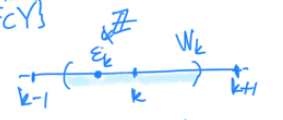
\includegraphics[scale=0.3]{images/ej_axiomas_num_real} 
    \end{center}
    \begin{demo}
        $\alpha = \mathbb{Z} \in Y,\ \exists \mathcal{W}^{\alpha} = \{W_k : k \ge 1\}$ abiertos saturados, $W_k \supset \mathbb{Z},\ \forall k$

        (figura) $\Rightarrow U = \mathbb{R} \setminus \{\varepsilon_k : k \ge 1\}$ entorno abierto saturado de $\mathbb{Z} U \not \supset W_k,\ \forall k$.
    \end{demo}

    \item $\forall$ aplicación continua y abierta conserva I y II [Imagen de base es base]
    \item $\forall $ aplicación continua conserva separabilidad [$f\left( \overline{A} \right) \subset \overline{f\left( A \right)}$]
    %TODO: Ya se sabe xd
    \item $\forall$ aplicación continua conserva Lindelöf [Como la compacidad, ya se sabe...]
\end{itemize}

\begin{itemize}
    \item Para productos: producto finito de numerables es numerable.
    \item Para sumas: suma finita de numerables es numerable.
    \item Solo falla Lindelöf:
    \begin{itemize}
        \item $\left( \mathbb{R}, \mathcal{T}_{[, )} \right)$ es Lindelöf [ejercicio no banal]
        \item $\left( \mathbb{R}^2, \mathcal{T}_{[, )}^2 \right)$ no es Lindelöf: si lo fuera, $L = \{x + y = 0\} \subset \mathbb{R}^2$ heredaría la propiedad, pero es \underline{discreto} no numerable ¡!
    \end{itemize}
\end{itemize}

\chapter{Compacidad}%
\label{cha:compacidad}
\section{Concepto y mantras}%
\label{sec:concepto_y_mantras_comp}
\begin{defi}
$X$ es \underline{compacto} si todo recubrimiento abierto tiene un subrecubrimiento finito:
\[
X = \bigcup_{i \in  I} U_i \Rightarrow \exists U_{i_1} \cup \ldots \cup U_{i_r} = X
\]
\end{defi}

\begin{obs}
Complementando lo anterior tenemos la \underline{propiedad de la intersección finita}: 
\begin{gather*}
    \emptyset = \bigcap_{i \in I} F_i \Rightarrow \exists F_{i_1} \cap \ldots \cap F_{i_r} = \emptyset \Rightarrow\\
    \forall F_{i_1} \cap \ldots \cap F_{i_r} \neq \emptyset \Rightarrow \bigcap_{i \in  I} F_i \neq \emptyset
.\end{gather*}
\end{obs}

\begin{prop}[Subespacios]
Sea $K \subset X$ (compacto) $\Rightarrow K \subset \underbrace{\bigcup_{i \in  I} U_i}_{\subset X} \Rightarrow \exists U_{i_1} \cup \ldots \cup U_{i_r} \supset K$
\end{prop}

\begin{ej}
\begin{enumerate}
    \item $K \subset \mathbb{R}_u^n$ es compacto $\Leftrightarrow K$ es cerrado y acotado (Heine-Borel). 
    \item $\left[ a, b \right] \subset \mathbb{R}_u$ compacto.
    \item Si es compacto y discreto $\Rightarrow$ es finito [$X = \bigcup_{x \in X} \{x\}$ es rec. abierto en $\mathcal{T}_{\text{discreta}}$]
    \item $x_k \rightarrow x \Rightarrow K = \{x, x_k: k \ge 1\}$ es compacto.
    \begin{demo}
        \[
            \exists U_{i_0} \ni x \xRightarrow{\lim} \begin{rcases}
                x_k \in U_{i_0},\ \forall k > k_0\\
                x_k \in U_{i_k},\ \forall k \le k_0
            \end{rcases} \Rightarrow K \subset U_{i_0} \cup U_{i_1} \cup \ldots \cup U_{i_{k_0}} 
        \]
    \end{demo}

    \item $K \subset \mathbb{R}_u^n$ compacto $\Leftrightarrow \forall A^{\infty} \subset K, A' \cap K \neq \emptyset$ (Bolzano-Weierstrass)
\end{enumerate}
\end{ej}

\begin{prop}[Mantra 1]
Cerrado en compacto es compacto. 
\end{prop}
\begin{demo}
Sea $K \stackrel{\text{cerr.}}{\subset} X$,
\begin{align*}
    K \subset \bigcup_{i} U_i &\Rightarrow X = \left( X \setminus K \right) \cup \bigcup_{i} U_i\\
    X \text{ comp.} &\Rightarrow \exists \left( X \setminus K \right) \cup U_{i_1} \cup \ldots \cup U_{i_r} = X \supset K\\
    &\Rightarrow U_{i_1} \cup \ldots \cup U_{i_r} \supset K
.\end{align*}

(Alternativa: Usar la propiedad de las intersecciones finitas)
\end{demo}

\begin{prop}[Mantra 2]
Infinito en compacto tiene puntos de acumulación.
\end{prop}
\begin{demo}
Sea $A \subset X$ (compacto) con $A' = \emptyset \Rightarrow$
\begin{align*}
    \overline{A} &= \overbrace{\{\text{puntos aislados}\}}^{\subset A}  \cup \overbrace{A'}^{= \emptyset} = \{\text{puntos aislados}\} = A\\
     &\Rightarrow A \stackrel{\text{cerr.}}{\subset} X \text{ comp.} \Rightarrow \underbrace{A}_{= \{\text{pts. aisl.}\}} \text{ es compacto y discreto} \Rightarrow \#A < +\infty   
.\end{align*}
\end{demo}

\begin{prop}[Mantra 3]
La imagen continua de un compacto es compacta. 
\end{prop}
\begin{demo}
Sea $f: X \rightarrow Y$ con $f$ continua y $X$ compacto $\Rightarrow$
\begin{align*}
    f\left( X \right) \times \bigcup_{i} V_i &\Rightarrow X = \bigcup_{i} f^{-1} V_i \Rightarrow \exists f^{-1}V_{i_1} \cup \ldots \cup f^{-1}V_{i_r} = X\\
     &\Rightarrow V_{i_1} \cup \ldots \cup V_{i_r} \supset f\left( X \right) 
.\end{align*}
\end{demo}

\begin{ej}[¡Muy importante!]
$\mathbb{R} \mathrm{P}^n$ es compacto: La imagen continua de $\mathbb{S}^n$ por la proyección antipodal. 
\end{ej}

\begin{prop}[Mantra 4]
Un compacto en $T_2$ es cerrado. 
\end{prop}
\begin{demo}
Sea $K \subset X$ con $K$ compacto y $X = T_2 \Rightarrow$
\begin{equation} \label{eq:mantra_4_1}
    \forall x \in X \setminus K,\ \exists U^x \cap U^k = \emptyset
\end{equation}
A su vez, $\forall y \in K,\ \exists U_y^x \cap U^y = \emptyset$ por $T_2 \Rightarrow$
\begin{align*}
    %TODO: Fix flecha
    K \subset \bigcup_{y} U^y &\xRightarrow{\text{comp.}} K \subset U^{y_1} \cup \ldots \cup U^{y_r} = U^k\\
    &\Rightarrow x \in U_{y_1}^x \cap \ldots \cap U_{y_r}^x = U^x
.\end{align*}
Finalmente, utilizando \ref{eq:mantra_4_1} $\Rightarrow$
\[
    U^x \subset X \setminus K\; \land \;X\setminus K \text{ es entorno de } x \Rightarrow X \setminus K \text{ abierto.} 
\]
%TODO: Imagen
\begin{center}
    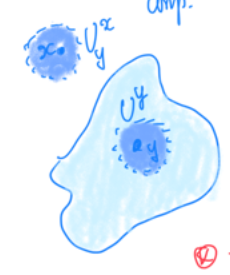
\includegraphics[scale=0.3]{images/mantra_4} 
\end{center}
\end{demo}
\begin{coro}
Dos compactos disjuntos en un $T_2$ se separan como puntos.
\end{coro}
\begin{demo}
    Ejercicio usando \ref{eq:mantra_4_1}.
\end{demo}

\begin{prop}
Si $f : X \rightarrow Y$ es continua, $X$ compacto e $Y = T_2 \Rightarrow$ cerrada.
\end{prop}
\begin{demo}
\[
    F \stackrel{\text{cerr.}}{\subset} X \xRightarrow{\mathrm{M}1} F \text{ comp.} \xRightarrow{\mathrm{M}3} f\left( F \right) \text{ comp.} \xRightarrow{\mathrm{M}4} f\left( F \right) \text{ cerr.} 
\]
\end{demo}
\begin{coro}
Sea la $f$ de la anterior proposición entonces si además es:
\[
\begin{cases}
    \text{inyectiva}\\
    \text{sobreyectiva}\\
    \text{biyectiva}
\end{cases} \Rightarrow
\begin{cases}
    \text{inmersión cerrada}\\
    \text{identificación cerrada}\\
    \text{homeomorfismo}
\end{cases} 
\]
\end{coro}

\section{Tabla de comportamiento}%
\label{sec:tabla_de_comportamiento_comp}
%TODO: Fix tabla
\begin{center}    
\begin{tabular}{c | c | c | c | c |}
& Subespacios & Cocientes & Productos & Sumas\\
\hline\\
    Compacidad & \begin{tabular}{@{}c@{}}$\times$\\ cerrados \checkmark \end{tabular} & \checkmark & \checkmark & \checkmark\\
    \hline\\
               & Mantra $1$ & Mantra $3$ & Tychonoff & Unión finita\\
    \hline\\
\end{tabular}
\end{center}

\begin{theo}[de Tychonoff]
Si $X$ e $Y$ son dos compactos $\Rightarrow X \times Y$ es compacto.
\end{theo}
\begin{demo}
Sea $X \times Y = \bigcup_{i \in  I} W_i,\ W_i \in \mathcal{T}_X \times \mathcal{T}_Y$.
\begin{enumerate}
    \item $\forall x\ \forall y,\ \exists U_y^x \times V_x^y \subset W_i$, $i$ depende de $\left( x, y \right)$.
    \item $\forall x\ Y = \bigcup_{y} V_x^y \xRightarrow{Y \text{comp.}} Y = V_x^{y_1} \cup \ldots \cup V_x^{y_r}$, los $y_k$ y su nº dependen de $x$.
    \item $U^x = U_{y_1}^x \cap \ldots \cap U_{y_r}^x,\ U^x \times V_x^{y_k} \subset W_{i_k}$, $i_k$ depende de $x$.
    \item $X = \bigcup_{x} U^x \xRightarrow{X \text{comp.}} X = U^{x_1} \cup \ldots \cup U^{x_s}$.
    \item 
    \[
        X \times Y = \bigcup_{\substack{l, k\\ \text{fin.}}} U^{x_l} \times V_{x_l}^{y_k} \subset \bigcup_{\substack{l, k\\ \text{fin.}}} W_{i_k} \text{, los } i_k \text{ dependen de los } x_l. 
    \]
\end{enumerate}
\end{demo}

\begin{obs}
\begin{enumerate}
    \item $X \times Y$ compacto $\Rightarrow X$ e $Y$ compactos. [Mantra $3$ para proyecciones] 
    \item Heine-Borel: $K \subset \mathbb{R}_u^n$ cerrado y acotado $\Rightarrow$ compacto porque:
    \[
        \exists a_i, b_i: K \stackrel{\text{cerr.}}{\subset} \underbrace{\left[ a_1, b_1 \right] \times \ldots \times \left[ a_n, b_n \right]}_{\text{Compacto por Tych.\footnotemark}}  
    \]
    \footnotetext{$\left[ a, b \right]$ es compacto.}
    Y aplicamos el Mantra $1$.
\end{enumerate}
\end{obs}

\chapter{Compacidad local}%
\label{cha:compacidad_local}
\begin{defi}
Sea $Y \subset X$, es \underline{localmente cerrado} si cumple las condiciones equivalentes siguientes:
\begin{enumerate}
    \item $\forall y \in Y,\ \exists U^y \subset X: Y \cap U^y \stackrel{\text{cerr.}}{\subset} U^y$. ($\Rightarrow$ lo mismo $\forall V^y \subset U^y$)
    \item $Y$ es abierto en su adherencia.
    \item $Y = F \cap U,\ F \stackrel{\text{cerr.}}{\subset} X,\ U \stackrel{\text{ab.}}{\subset} X$. ($\Rightarrow$ vale $F = \overline{Y}$)
\end{enumerate}
\end{defi}
\begin{demo}
\begin{enumerate}
    \item[1. $\Rightarrow$ 2.)] $Y = \overline{Y} \cap \left( \bigcup_{y \in Y} U^y \right)$:
    \begin{align*}
        x \in \overline{Y} \cap U^y &\Rightarrow x \in \adh_{U^y} \left( Y \cap U^y \right) = Y \cap U^y \subset Y\\
        U^x \subset U^y &\Rightarrow \emptyset \neq Y \cap U^x = \left( Y \cap U^y \right) \cap U^x
    .\end{align*}
    \item[2. $\Rightarrow$ 3.)] Abierto en $\overline{Y} = \underbrace{\overline{Y}}_{= F} \cap U$.
    \[
    F \cap U = Y \Rightarrow F \supset \overline{Y} \Rightarrow F \cap U = \overline{Y} \cap U.
    \]
    \item[3. $\Rightarrow$ 1.)] $Y = F \cap U \stackrel{\text{cerr.}}{\subset} U \left( = U^y,\ \forall y \right)$.
\end{enumerate}
\end{demo}

Esto es un ejemplo de \underline{localización} de una propiedad topológica $\mathcal{P}$ (aquí es ser cerrado). Se puede entender como:
\begin{align*}
    &\forall x,\ \exists V^x \text{ que cumple } \mathcal{P} \text{ o } \\
    &\forall x,\ \exists \mathcal{V}^x \text{ base de entornos que cumplen } \mathcal{P} 
.\end{align*}
A veces son equivalentes (como en este caso), a veces no. El concepto adecuado de localización es mediante \underline{bases de entornos}.

\section{Compacidad local y mantras}%
\label{sec:compacidad_local_y_mantras}
\begin{defi}
$X$ es \underline{localmente compacto} si $\forall x \in X,\ \exists \mathcal{V}^x$ base de entornos compactos.
\end{defi}

\begin{ej}
\begin{enumerate}
    \item $\mathbb{R}_u^n$ es localmente compactos: $\mathcal{V}^x = \{B\left[ x, \varepsilon \right] : \varepsilon > 0\}$

    \item $T = B\left( 0, 1 \right) \cup \{p\},\ T_u$ no es compacto:
    \begin{align*}
        \exists V^p \stackrel{\text{comp.}}{\subset} T &\Rightarrow \exists B\left( 0, \varepsilon \right) \cap T \subset V^p \Rightarrow \exists \overbrace{x_k}^{\in V^p} \rightarrow x_0 \in S\left( 0, 1 \right) \setminus T\\
       &\Rightarrow \{x_k : k \ge 1\} \subset V^p \subset T 
    .\end{align*}
    que es un conjunto infinito sin acumulación en $T$.
    %TODO: Imagen
    \begin{center}
        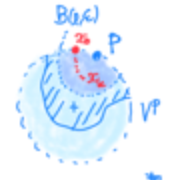
\includegraphics[scale=0.3]{images/loc_comp_ej_2} 
    \end{center}

    \item En general \underline{no} basta que exista un entorno compacto.

    %TODO: no sé que pone
    En $S = T \cup \{q\}?$ tomamos como entornos del punto añadido $q$ los $W \subset S$ que tienen complementario finito (y $q \in W$).

    Pero este caso es un ejemplo con un espacio \underline{no separado}.
\end{enumerate}
\end{ej}

\begin{prop}
Si $X$ es $T_2$ y $x \in X$ tiene un entorno compacto, entonces tiene una base de entornos compactos.
\end{prop}
\begin{demo}
    $\exists \underbrace{V^x}_{\supset W^x \text{ab.}}$ compacto $\Rightarrow \mathcal{V}^x =$ { entornos compactos $K^x$} \underline{base de entornos}: $\forall U^x,\ \exists?K^x \subset U^x$.

    $\exists_{\text{ab.}} U_1^x \subset \overline{U_1^x} \subset U^x$:
    \begin{gather*}
        V^x\setminus U^x \stackrel{\text{cerr.}}{\subset} V_{\text{comp.}}^x \Rightarrow \overbrace{V \setminus U}^{\not\ni x} \text{comp. en } T_2 \Rightarrow \exists \overbrace{U_1^x\ \&\ A}^{\text{ab. disjuntos}} \supset V^x \setminus U^x\\
        K^x = \overline{W^x \cap U_1^x} \begin{cases}
            %TODO: Anotación
            \overline{V^x} \cap \overline{U_1^x} = V^x \cap \overline{U_1^x} \subset V^x \cap \overline{X \setminus A} = V^x \cap \overbrace{\left( X \setminus A \right)}^{\text{cerr.}} \subset U^x\\
            \text{interdos ent.?} \Rightarrow \text{entorno}\\
            W^x \cap U_1^x \subset V^x \stackrel{\text{comp. en } T_2}{=} \overline{V^x} \subset X \Rightarrow \underbrace{K^x}_{\text{cerr.}} \subset \underbrace{V^x}_{\text{comp.}} \Rightarrow K^x \text{ comp.} 
        \end{cases}  
    \end{gather*}
\end{demo}

Y tenemos dos mantras:
\begin{prop}[Mantra 1]
Localmente cerrado en localmente compacto es localmente compacto. 
\end{prop}
%TODO: Arreglar formato
\begin{demo}
    Sea $Y \subset X$ con $Y$ loc. cerrado y $X$ loc. compacto e $y \in Y$.

    Tenemos:
    \[
    \overline{U_1^x} \cap V^x \subset \overline{X \setminus A} \cap V^x = \overbrace{\left( X \setminus A \right)}^{\text{cerr.}} \cap V^x \subset U^x
    \]

    Y como $Y$ es loc. cerrado, $\exists W^y \cap Y \stackrel{\text{cerr.}}{\subset} W^y$ ent. en $X$. Por ser $X$ loc. compacto $\exists K^y$ compacto tal que, $K^y \subset W^y \Rightarrow K^y \cap W^y \cap Y \stackrel{\text{cerr.}}{\subset} K^y \Rightarrow$
    \[
    L^y = \underbrace{K^y \cap W^y}_{\text{ent. en } X} \cap Y \stackrel{\text{cerr.}}{\subset} K^y \Rightarrow L^y \text{ ent. en } Y \text{ compacto.}  
    \]
\end{demo}

\begin{prop}[Mantra 2]
Localmente compacto en $T_2$ es localmente compacto.
\end{prop}
\begin{demo}
Sea $Y \subset X$ con $Y$ loc. compacto, $X$ siendo $T_2$ e $y \in Y \Rightarrow$
\[
\underbrace{\exists L^y}_{\text{comp.}} = \underbrace{V \cap Y}_{\text{ent. en } Y} \subset \underbrace{V}_{\text{ent. en } X} \xRightarrow{T_2} V \cap Y = L^y \stackrel{\text{cerr.}}{\subset} V.
\]
\end{demo}

\section{Tabla de comportamiento}%
\label{sec:tabla_de_comportamiento_loc_comp}
%TODO: Fix tabla
\begin{center}    
\begin{tabular}{c | c | c | c | c |}
& Subespacios & Cocientes & Productos & Sumas\\
\hline\\
    Compacidad local & \begin{tabular}{@{}c@{}}$\times$\\ Loc. cerrados \checkmark \end{tabular} & \begin{tabular}{@{}c@{}}$\times$\\ ab. \checkmark \end{tabular} & \checkmark & \checkmark\\
    \hline\\
           & Mantra $1$ & $f\left( \text{ent.} \right) = $ ent & Tychonoff & Loc. suma es como sum's\\
    \hline\\
\end{tabular}
\end{center}

\begin{ej}
$Y = \mathbb{R} / \mathbb{Z}$ no es localmente compacto.
\begin{enumerate}
    \item $\mathbb{Z} \subset \underbrace{W}_{\text{ab.}} \subset \mathbb{R}: \exists k + \underbrace{\varepsilon_k}_{0 < \varepsilon_k < 1} \in W\ \forall k \ge 1 \Rightarrow A = \{k + \varepsilon_k : k \ge 1\} \subset W$
    \begin{itemize}
        \item Cerrado
        \item Saturado ($n\mathbb{Z} = \emptyset$)
        \item Infinito
        \item Discreto
    \end{itemize}

    \item $\exists K \subset Y$ entorno compacto de $y = \mathbb{Z} \in Y \Rightarrow \exists \underbrace{W^{\text{ab.}}}_{\supset \mathbb{Z}} \subset p^{-1} K \Rightarrow pA \subset K$ infinito sin acumulación.
\end{enumerate}
\end{ej}

\section{Compactificación por un punto}%
\label{sec:compactificacion_por_un_punto}
Este es otro problema importante: \underline{sumergir un espacio} como subespacio abierto denso de un espacio compacto.

Intuitivamente se trata de añadir los límites que el espacio no tiene (por no ser compacto).

\begin{ej}
\begin{enumerate}
    \item $\mathbb{R}^n \equiv B^n \setminus \{a\} \subset \mathbb{S}^n$ vía proyección estéreo desde $a$.
    \item $\mathbb{R}^n \equiv \mathbb{R}P^n \setminus H \subset \mathbb{R}P^n$ vía cartas afines.
\end{enumerate}
\end{ej}

\begin{prop}
$X$ localmente compacto $T_2$.
\begin{enumerate}
    \item $\exists j : X \xhookrightarrow{} X^*$ comp. $T_2,\ j$ inmersión abierta $X^* \setminus j\left( X \right) = \{w\}$.
    \item Unicidad: 
    \begin{center}
        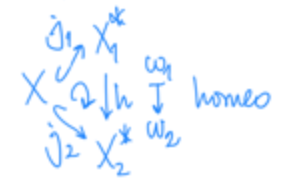
\includegraphics[scale=0.3]{images/comp_pto_prop_1} 
    \end{center}
\end{enumerate}
\end{prop}
\begin{demo}
\begin{enumerate}
    \item $X^* = X \cup \{0\},\ \mathcal{T}^* = \mathcal{T} \cup \{X^* \setminus K: \overbrace{K}^{\subset X} \text{comp.}\}$.
    \begin{itemize}
        \item $\mathcal{T}^*$ es top: fácil por las hipótesis sobre $X$.
        \begin{itemize}
            \item $K_i \stackrel{\text{comp.}}{\subset} X \xRightarrow{T_2} K_i \stackrel{\text{cerr.}}{\subset} X \Rightarrow \overbrace{\bigcap_{i} K_i}^{\text{cerr.}} \subset \overbrace{K_{i_0}}^{\text{comp.}} \Rightarrow \bigcap_{i} K_i$ comp.
            \item $U \stackrel{\text{ab.}}{\subset} X,\ X \stackrel{\text{comp.}}{\subset} X \Rightarrow U \setminus K =$ ab. $\setminus$ cerr. $ = $ ab.
            \item $U \stackrel{\text{ab.}}{\subset} X,\ K \stackrel{\text{comp.}}{\subset} X \Rightarrow U \cup \left( X^* \setminus K \right) = X^* \setminus \left( K \setminus U \right),\ K \setminus U \subset K$ cerrado $\Rightarrow$ compacto.
        \end{itemize}
        \item $X \subset X^*$ inmersión abierta: $\left( X^* \setminus K \right) \cap X = X \setminus K \in \mathcal{T}$ pues $X$ es $T_2$.
        \item $X^*$ es compacto: $X^* = \bigcup_{i} W_i$.
        \[
        \exists W_{i_0} \ni w \Rightarrow W_{i_0} = \underbrace{X^* \setminus K}_{\text{comp.}} \Rightarrow K \subset W_{i_1} \cup \ldots \cup W_{i_r} \Rightarrow X^* = W_{i_0} \cup W_{i_1} \cup \ldots \cup W_{i_r}  
        \]
        \item $X^*$ es $T_2:$
        \[
        x \in X \text{ loc. comp.} \Rightarrow \exists K^x \text{ ent. comp.} \Rightarrow X^* \setminus K^* = U^w \text{ ent. de } w
        \]
    \end{itemize}

    \item Unicidad:
    \begin{itemize}
        \item $\begin{rcases}
           h_{j_1} = j_2\\
           j_i \text{ inmersiones} 
        \end{rcases} \Rightarrow h|: j_1\left( X \right) \rightarrow j_2 \left( X \right)$ homeomorfismo.

        \item $h$ continua en $w_1$ (análogamente $h^{-1}$ continua en $w_2$)
        \begin{align*}
            h\left( w_1 \right) = w_2 \in W \stackrel{\text{ab.}}{\subset} X_2^* &\Rightarrow X_2^* \setminus W \stackrel{\text{cerr.}}{\subset} X_2^* \Rightarrow X_2^* \setminus W \stackrel{\text{comp.}}{\subset} j_2\left( X \right)\\
            &\Rightarrow K = h^{-1}\left( X_2^* \setminus W \right) \stackrel{\text{comp.}}{\subset} j_1\left( X \right) \subset X_1^*\\
            \left[ X_1^* \text{ es } T_2 \right] &\Rightarrow K \stackrel{\text{cerr.}}{\subset} X_1^* \Rightarrow h^{-1}\left( W \right) = X_1^* \setminus K \stackrel{\text{ab.}}{\subset} X_1^*
        .\end{align*}
    \end{itemize}
\end{enumerate}
\end{demo}

\begin{defi}
El espacio $X^*$ se denomina \underline{compactificación por un punto} de $X$. 

También, \underline{compactificación de Alexandroff}.
\end{defi}
Por ejemplo, $\mathbb{S}^n$ es la compactificación por un puntoo de $\mathbb{R}^n$ (vía proyección estéreo como dijimos antes).

\begin{obs}[¡Importante!]
\begin{enumerate}
    \item La unicidad justifica? que un espacio $X^*$ compacto $T_2$ es la compactificación de $X^* \setminus \{0\}$ para cualquier $w \in X^*$.

    \item Si dos espacios son homeomorfos, lo son sus compactos.
    \[
        X_1 \xrightarrow[\text{homeo.}]{f} X_2 \xhookrightarrow{j_2} X_2^* \Rightarrow j_1 = j_2 \circ f : X_1 \rightarrow X_2^*
    \]
    que cumple las condiciones.

    \item Si dos espacios no son homeomorfos, pueden serlo sus compactos.
    \begin{center}
        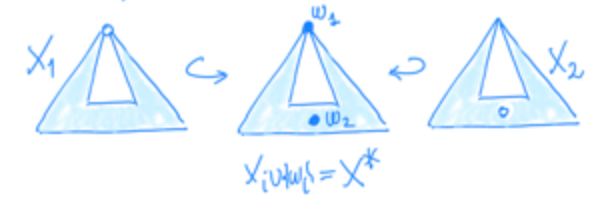
\includegraphics[scale=0.3]{images/obs_comp_pto} 
    \end{center}
\end{enumerate} 
\end{obs}

[\underline{Ejercicio}: $\mathbb{R}_u^2$: ¿Por qué $X_1 \not \approx X_2$?]

\chapter{Conexión}%
\label{cha:conexion}
\section{Concepto y mantras}%
\label{sec:concepto_y_mantras_conx}
\begin{defi}
$X$ es \underline{conexo} si cumple las siguientes condiciones equivalentes:
\begin{enumerate}
    %TODO: union rara
    \item $\nexists X = U \sqcup Y$ abiertos $\neq \emptyset$.
    \item $\nexists X = F \sqcup C$ cerrados $\neq \emptyset$.
    \item $\nexists E \subsetneq X$ abierto y cerrado $\neq \emptyset$.
\end{enumerate}
\end{defi}
\begin{demo}
Equivalencia: $F = X \setminus V,\ C = X \setminus U,\ E = U = X \setminus V.$
\end{demo}

\begin{obs}
$Y \subset X$ subespacio conexo: $\nexists Y \subset U \cup V$ abierto de $X$, 
\[
\begin{cases}
    U \cap Y \neq \emptyset\\
    V \cap Y \neq \emptyset\\
    U \cap V \cap Y = \emptyset
\end{cases} 
\]
\end{obs}

\begin{ej}[Fundamental]
$\left( 0, 1 \right) \subset \mathbb{R}_u$ es conexo. 

Mantras generales $\Rightarrow$ segmentos en $\mathbb{R}^n$, estrellados? y conexos son conexos.
\end{ej}

\begin{theo}[del pivote. Mantra 1] 
Sea $X = \bigcup_{i} A_i,\ \bigcap_{i} A_i \neq 0,\ \forall A_i$ conexos $\Rightarrow X$ conexos.
\end{theo}
\begin{demo}
\begin{align*}
    \emptyset \neq E \stackrel{\text{ab. cerr.}}{\subset} X &\Rightarrow \forall i,\ E \cap A_i \stackrel{\text{ab. cerr.}}{\subset} A_i \Rightarrow \forall i,\ \begin{cases}
        E \cap A_i = \emptyset\\
        E \supset A_i
    \end{cases}\\
    &\xRightarrow{E \neq \emptyset} \exists i_0: E \supset A_{i_0} \supset \bigcap_{i} A_i \neq \emptyset \Rightarrow \forall i,\ E \cap A_i \neq \emptyset \Rightarrow \forall i,\ E \supset A_i\\
    &\Rightarrow E \supset \bigcup_{i} A_i \Rightarrow E = X
.\end{align*}
\end{demo}

\begin{coro}[Variantes]
\begin{enumerate}
    \item $X = \bigcup_{i \in  I} A_i,\ \exists A_{i_0} \cap A_i \neq \emptyset$.
    \begin{demo}
        $X = \bigcup_{i \in  I}\left( A_{i_0} \cup A_i \right)$ conexo por mantra $1$ y se aplica el mantra $1$.
    \end{demo}
    \item Cadenas: $X = \underbrace{A_1 \cup \ldots \cup A_k \cup \ldots}_{\text{conexos}}\quad A_k \cap A_{k + 1} \neq \emptyset \Rightarrow X$ conexo.
    \begin{demo}
        Se usa el mantra $1$ dos veces:
        \[
        \begin{cases}
            X_k = \left( \ldots \left( \left( A_1 \cup A_2 \right) \cup A_3 \right) \cup \ldots \cup \right) A_k\\
            X = \bigcup_{k} \left( X_1 \cup \ldots \cup X_k \right) 
        \end{cases} 
        \]
        %TODO: Imagen
        \begin{center}
            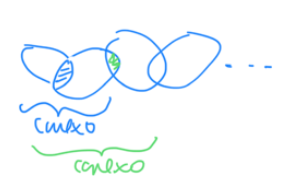
\includegraphics[scale=0.3]{images/dem_var_mantra_1_conx} 
        \end{center}
    \end{demo}
\end{enumerate} 
\end{coro}

El ``recíproco'' es ``fácil'' pero útil.
\begin{prop}[Construcción de cadenas]
$X$ conexo, $X = \bigcup_{i} U_i$ recubrimiento abierto, $p, q \in X \Rightarrow \exists$ cadena finita $U_{i_k}$ de $p$ a $q: p \in U_{i_0}, U_{i_{k - 1}} \cap U_{i_k} \neq \emptyset,\ q \in U_{i_r}$. 
\end{prop}
\begin{demo}
$A = \{x \in X: \exists U_{i_k} \text{ de } p \text{ a } x\} \neq \emptyset$ abierto y cerrado $\Rightarrow A = X$ y $q \in A$. Por ser:
\begin{itemize}
    \item $\neq \emptyset: \exists U_{i_0} \in? p$ y $U_{i_0}$ va de $p$ a $p$ !
    \item Abierto: $\exists U_{i_0}, \ldots, U_{i_r}$ de $p$ a $x \Rightarrow U_{i_r} \subset A$.
    \item Cerrado: 
    \begin{align*}
        y \in \overline{A} \text{ e } y \in U_{i\left( y \right)} &\Rightarrow A \cap U_{i\left( y \right)} \neq \emptyset\\
        &\Rightarrow \exists U_{i_0}, \ldots, U_{i_r} \text{ de } p \text{ a } x\in U_{i\left( y \right)}\\
        &\Rightarrow U_{i_0}, \ldots, U_{i_r}, U_{i\left( y \right)} \text{ de } p \text{ a } y
    .\end{align*}
\end{itemize}
%TODO: Imagen
\begin{center}
    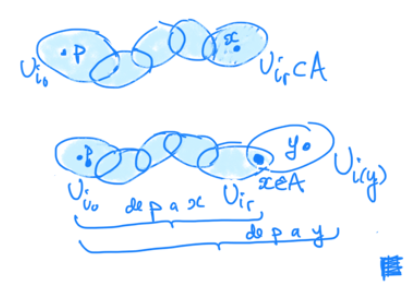
\includegraphics[scale=0.3]{images/dem_const_cadenas} 
\end{center}
\end{demo}

\begin{prop}[Mantra 2]
Imagen continua de conexo es conexo. 
\end{prop}
\begin{demo}
    $f: X \rightarrow Y$ continua, $\emptyset \neq E \stackrel{\text{ab. cerr.}}{\subset} f\left( X \right) \xRightarrow{\text{cont.}} \emptyset \neq f^{-1}\left( E \right) \stackrel{\text{ab. cerr.}}{\subset} X \Rightarrow f^{-1}\left( E \right) = X \Rightarrow E = f\left( X \right)$.
\end{demo}

\begin{prop}[Mantra 3]
Adherencia de conexo es conexo: $Y \subset X$ con $Y$ conexo y denso $\Rightarrow X$ conexo. 
\end{prop}
\begin{demo}
    $\emptyset \neq E \stackrel{\text{ab. cerr.}}{\subset} X \Rightarrow E \cap Y \stackrel{\text{ab. cerr.}}{\subset} Y \Rightarrow \begin{cases}
        E \cap Y = \emptyset\ \times \text{densidad.} \\
        E \cap Y = Y \Rightarrow Y \subset E \stackrel{\text{cerr.}}{\subset} X = \overline{Y} \Rightarrow E = X.
    \end{cases}$
\end{demo}

\begin{ej}
   %TODO: Ejemplos complicados
    \begin{enumerate}
        \item $\left( 0, 1 \right) \stackrel{\text{denso}}{\subset} \left[ 0, 1 \right] \xRightarrow{\mathrm{M}1} \Rightarrow \left[ 0, 1 \right]$ conexo. Con una interpolación?: $\sigma\left( t \right) = \left( 1 - t \right) a + tb$ es homeomorfismo con $\left[ a, b \right] \subset \mathbb{R}^n \xRightarrow{\mathrm{M}2} \left[ a, b \right]$ es conexo. Aplicando ahora:
        \begin{itemize}
            \item Pivote: $E = \bigcup_{\substack{x \in E\\ \text{conx.}}} \left[ a, x \right]$ \underline{estrellado} (resp. de $a$): convexos, bolas abiertas y cerradas, rectángulos... 
            \item Mantra $2$: Trazas de curvas continuas $\sigma: \left[ 0, 1 \right] \rightarrow \mathbb{R}^n$.
        \end{itemize}
        \item \underline{Seno del topólogo} (polaco):

        Conexos: $\begin{cases}
            \Gamma = \text{imagen} : t \mapsto \left( t, \sin \frac{1}{t} \right),\ t > 0\\
            J = \{0\} \times \left[ 0, 1 \right]\\
            \overline{\Gamma} = \Gamma \cup J \text{ (adh.)} 
        \end{cases}$
        \begin{center}
            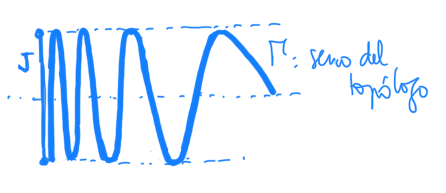
\includegraphics[scale=0.3]{images/seno_topologo} 
        \end{center}
    \end{enumerate}
\end{ej}

\section{Tabla de comportamiento}%
\label{sec:tabla_de_comportamiento_conx}
%TODO: Fix tabla
\begin{center}    
\begin{tabular}{c | c | c | c | c |}
& Subespacios & Cocientes & Productos & Sumas\\
\hline\\
    Conexión & $\times$ & \checkmark & \checkmark & $\times$\\
    \hline\\
               & $\{0, 1\} \subset \left[ 0, 1 \right]$ & Mantra $3$ & Pivote & Cada sum. ab. y cerr.\\
    \hline\\
\end{tabular}
\end{center}

\begin{prop}
$X \times Y$ conexo $\Leftrightarrow X$ y $Y$ conexo.
\end{prop} 
\begin{demo}
$\Rightarrow)$ Mantra $3$ para las proyecciones.

$\Leftarrow)$ Fijamos $a \in X$.
\begin{gather*}    
\forall y \in Y,
\begin{rcases}
    Z_y = \underbrace{\left( X \times \{y\} \right)}_{\approx X}\cup \underbrace{\left( \{a\} \times Y \right)}_{\approx Y} \text{ dos conx. se cortan en } \left( a, y \right) \xRightarrow{\text{Piv.}} Z_y \text{ conx.}\\
    \bigcap_{y \in Y} Z_y = \{a\} \times Y \neq \emptyset
\end{rcases} \xRightarrow{\text{Piv.}} \\
\bigcup_{y \in Y} Z_y = X \times Y \text{ conx.} 
\end{gather*}
%TODO: Imagen
\begin{center}
    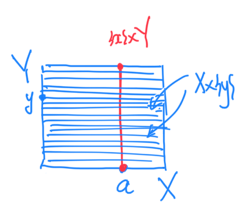
\includegraphics[scale=0.3]{images/dem_conx2_conx} 
\end{center}
\end{demo}

\chapter{Componentes conexas y conexión local}%
\label{cha:componentes_conexas_y_conexion_local}
\section{Componentes}%
\label{sec:componentes}
\begin{defi}
Una \underline{componente conexa} (c.c) de $X$ es un subespacio conexo maximal.
\end{defi}

\begin{prop}
\begin{enumerate}
    \item $\forall a \in X.\ C\left( a \right) = \bigcup_{a \in A \text{conx.}} A$ es conexo (pivote), $a \in C\left( a \right)$.
    \item $E \subset X$ conexo: 
    \[
    C\left( a \right) \cap E \neq \emptyset \Rightarrow C\left( a \right) \cup E \text{ conx. (pivote)} \Rightarrow C\left( a \right) \cup E \text{ es uno de los } A \text{ de } C\left( a \right) \Rightarrow E \subset C\left( a \right) 
    \]
    Luego, 
    \begin{itemize}
        \item $C\left( a \right)$ maximal $\Rightarrow$ componente conexa.
        \item $a \neq b: C\left( a \right) = C\left( b \right)$ ó $C\left( a \right) \cap C\left( b \right) = \emptyset$ [Usar $E = C\left( b \right)$]
    \end{itemize}

    \item $\overline{C\left( a \right)}$ conexo (mantra adh.) $\Rightarrow \overline{C\left( a \right)} = \underbrace{C\left( a \right)}_{\text{cerr.}}$ (maximalidad)
    %TODO: Fix
    \item[1. + 2. + 3.] $\Rightarrow X = \bigsqcup_{C \stackrel{\text{c.c}}{\subset}  X} C$ es una \underline{partición} en cerrados disjuntos.
\end{enumerate} 
\end{prop}

\begin{ej}
\begin{enumerate}
    \item $X_{\text{discreto}}: C\left( x \right) = \{x\}$ (puntos abiertos y cerrados)
    \item $\mathbb{Q}_u : C\left( p \right) = \{p\}$ (todo intervalo de $\mathbb{R}$ tiene racionales)
    \item $\left( \mathbb{R}, \mathcal{T}_{[, )} \right): C\left( t \right) = \{t\}$ ($\mathbb{R} = \left( \leftarrow, a \right) \cup \left[ a, \rightarrow \right)$ abierto y cerrado)
    \item $X = \{0, Y_k,\ k \ge 1\} : \begin{cases}
        C\left( 0 \right) = \{0\} \text{ cerrado, no abierto} \left( \{\frac{1}{k}: k\ge 1 \}  \text{ no cerr.}\right)\\
        C\left( \frac{1}{k} \right) = \{\frac{1}{k}\} \text{ cerrado y abierto.} 
    \end{cases} $
\end{enumerate}
\end{ej}

\begin{defi}
Un espacio cuyas componentes son los puntos se llama \underline{totalmente disconexo}. 
\end{defi}

\begin{prop}
Las componentes conexas de $X \times Y$ son los puntos de componentes conexas.
\end{prop}
\begin{demo}
$C \subset \underbrace{X}_{\xrightarrow{p} X} \times \underbrace{Y}_{\xrightarrow{q} Y} \Rightarrow p\left( C \right)$ y $q\left( C \right)$ conexos (imagen continua) $\Rightarrow \begin{cases}
    p\left( C \right) \subset E \stackrel{\text{c.c}}{\subset}  X\\
    q\left( C \right) \subset F \stackrel{\text{c.c}}{\subset}  Y
\end{cases} \Rightarrow C \subset E \times F \xRightarrow{\text{Max. de} C} C = E\times F$.
\end{demo}

\section{Conexión local}%
\label{sec:conexion_local}
\begin{defi}
$X$ es \underline{localmente conexo}  si $\forall x \in X,\ \exists \mathcal{B}^x$ base de entornos abiertos conexos.
\end{defi}

\begin{prop}
$X$ es localmente conexo $\Leftrightarrow$ la componente conexa de un abierto es abierta.
\end{prop}
\begin{demo}
\begin{itemize}
    \item $\Rightarrow)$ Si $x \in C \stackrel{\text{cerr.}}{\subset} U \stackrel{\text{ab.}}{\subset} X \Rightarrow \exists \underbrace{U^x}_{\text{ab. conx.}} \subset U \Rightarrow U^x \subset C \Rightarrow C \stackrel{\text{ab.}}{X}$.
    \item $\Leftarrow)\ \mathcal{B}^x = \{C\left( x \right) \stackrel{\text{c.c}}{\subset} U \stackrel{\text{ab.}}{\subset} X : x \in U\}$. Con $C\left( x \right)$ abierto por ser c.c de abierto.
\end{itemize}
\end{demo}

\underline{Ejercicio}: $X$ es localmente conexo $\Leftrightarrow \forall x \in X,\ \exists \mathcal{V}^x$ base de entornos conexos.

\begin{ej}[Esencial]
$\{0, \frac{1}{k} : k \ge 1\} = Y \subset \mathbb{R}_u$ \underline{no} es localmente conexo. 
\begin{demo}
    La $\text{c.c}\left( 0 \right) = \{0\}$ no es abierto. Directamente:
    \begin{align*}
        0 \in \underbrace{V}_{\text{ent. de } 0 \in \mathbb{R}} \cap Y &\Rightarrow V \supset \left( 0, \varepsilon \right),\ \exists 0 < \underbrace{\theta}_{\not\in \mathbb{Q}} < \frac{1}{k} < \varepsilon < 1\\
        &\Rightarrow V\cap Y \subset \underbrace{\left( \leftarrow, \theta \right)}_{\ni 0} \cup \underbrace{\left( \theta, \rightarrow \right)}_{\ni \frac{1}{k}}  \Rightarrow V \cap Y \text{ no conexo.} 
    .\end{align*}
\end{demo}
\end{ej}

\underline{Ejercicio}:
\begin{enumerate}
    \item Analizar una sucesión de segmentos que convergen a otro:
    \begin{center}
        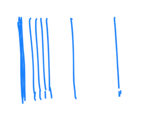
\includegraphics[scale=0.3]{images/suc_conv_otro} 
    \end{center}
    \item ¿Y el seno del topólogo?
\end{enumerate}

\section{Tabla de comportamiento}%
\label{sec:tabla_de_comportamiento_loc_conx}
%TODO: Fix tabla
\begin{center}    
\begin{tabular}{c | c | c | c | c |}
& Subespacios & Cocientes & Productos & Sumas\\
\hline\\
    Conexión local & $\times$ & \checkmark & \checkmark & $\times$\\
    \hline\\
               & Ejemplo esencial & No banal & Prod. ent. conx. & Suma como sum's\\
    \hline\\
\end{tabular}
\end{center}


\begin{prop}
Sea $f : X \rightarrow Y$ identificación con $X$ localmente conexo $\Rightarrow Y$ es localmente conexo.
\end{prop}
\begin{demo}
    El diagrama siguiente resume el argumento (si se lee en el orden adecuado).
    \begin{center}
        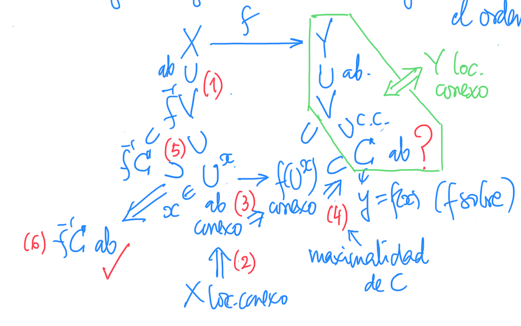
\includegraphics[scale=0.3]{images/dem_loc_conx_loc_conx} 
    \end{center}
\end{demo}

\chapter{Conexión por caminos}%
\label{cha:conexion_por_caminos}
\begin{defi}
Un \underline{camino} en un espacio $X$ es una aplicación continua $\alpha: \left[ a, b \right] \subset \mathbb{R}_u \rightarrow X$. Decimos:
\begin{itemize}
    \item $\alpha$ \underline{va de} $\alpha\left( a \right)$ a $\alpha\left( b \right)$, \underline{conecta} $\alpha\left( a \right)$ con $\alpha\left( b \right)$, que son \underline{extremos}.
    \item La imagen $\alpha\left[ a, b \right] \subset X$ es la \underline{traza}, conexa por imagen continua.
\end{itemize}
\end{defi}

\begin{prop}[Cambios de parámetros]
$\forall \varphi: \left[ c, d \right] \rightarrow \left[ a, b \right]$ continua $\Rightarrow \beta = \alpha \circ \varphi$ es otro camino con igual traza.    

$\varphi$ es un \underline{cambio de parámetro} cuando es homeomorfismo (creciente o decreciente).
%TODO: Imagen
\begin{center}
    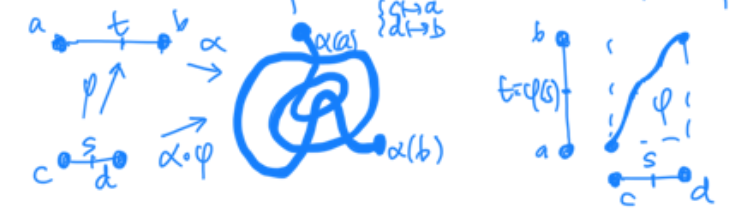
\includegraphics[scale=0.3]{images/camb_par_caminos} 
\end{center}
\end{prop}

\begin{ej}[Interpolación lineal]
Dados $p, q \in \mathbb{R}^n,\ \alpha : \left[ 0, 1 \right] \rightarrow \left[ p, q \right]: t \mapsto \left( 1 - t \right) p + tq$ es un camino bien conocido y útil. También sirve para reparametrizar si $\left[ p, q \right] = \left[ a, b \right] \subset \mathbb{R}$. Vemos, por ejemplo, que siempre podemos reducirnos a caminos con dominio $\left[ 0, 1 \right]$. Esto será fundamental más adelante. 
\end{ej}

\begin{prop}[Producto de caminos]
Topológicamente: 
%TODO: Imagen
\begin{center}
    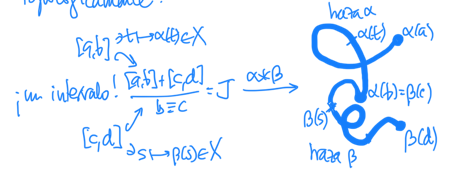
\includegraphics[scale=0.3]{images/prod_caminos} 
\end{center}
(Alternativa: Reparametrizar $\beta$ con dominio $\left[ b, b + \left( d - c \right) \right]$)
\end{prop}

\begin{ej}
Si hacemos el producto de segmentos consecutivos obtenemos \underline{caminos poligonales}. 
\end{ej}

\section{Conexión por caminos}%
\label{sec:conexion_por_caminos}
\begin{defi}
Un espacio $X$ es \underline{conexo por caminos} si sus puntos se pueden conectar con un camino:
\[
\forall x \forall y \in X,\ \exists \sigma_y: \left[ a, b \right] \rightarrow X,\ \sigma_y\left( a \right) = x\; \land \;\sigma_y\left( b \right) = y
\]
En particular, $X = \bigcup_{y} \sigma_y\left[ a, b \right]$ es \underline{conexo} (pivote, $\alpha_y\left( a \right) = x,\ \forall y$)
\end{defi}

\begin{ej}
\begin{enumerate}
    \item La mayor parte de los conexos conocidos son conexos por caminos:
    \begin{itemize}
        \item Los abiertos conexos (top. Usual) son conexos por poligonales, que son caminos.
        \item Los conjuntos convexos y los estrellados también.
    \end{itemize}
    \item El seno del topólogo $\Gamma$ es la traza de $\alpha\left( t \right) = \left( t, \sin\frac{1}{t} \right),\ t > 0$, es conexo y lo es su adherencia $\overline{\Gamma} = J \cup \Gamma,\ J = \{0\} \times \left[ 0, 1 \right]$. Pero $\overline{\Gamma}$ \underline{no} es conexo por caminos.
    \begin{demo}
        No existen caminos $\sigma: \left[ a, b \right] \rightarrow \overline{\Gamma} \begin{cases}
            \sigma\left( a \right) = p \in J\\
            \sigma\left( b \right) = q \in \Gamma
        \end{cases}$:
        \begin{center}
            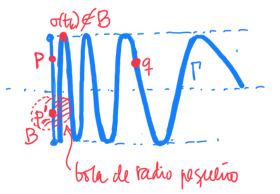
\includegraphics[scale=0.3]{images/dem_sin_top_no_conx_caminos} 
        \end{center}
        \begin{enumerate}
            \item $\sigma\left( t \right) = \left( \alpha\left( t \right), \beta\left( t \right) \right),\ \alpha, \beta$ continuas. $\exists a' = \max \{t \in \left[ a, b \right] : \alpha\left( t \right) = 0\} \Rightarrow (\alpha$ continua en un compacto) %TODO: Fix orden 
            $\Rightarrow \begin{cases}
                \alpha\left( a' \right) = 0,\ \sigma\left( a' \right) = p' \in J\\
                t > a': \alpha\left( t \right) > 0 \Rightarrow \sigma\left( t \right) \in \Gamma \Rightarrow \beta\left( t \right) = \sin \frac{1}{\alpha\left( t \right)} 
            \end{cases} $

            \item Supongamos $p' = \sigma\left( a' \right) \neq \left( 0, 1 \right)$ y $\exists \delta: B\left( p', \delta \right) \cap \{y = 1\} = \emptyset$. $\sigma$ continua $\Rightarrow \exists \sigma\left[ a', \varepsilon \right] \subset B\left( p', \delta \right) \Rightarrow \sigma\left[ a', \varepsilon \right] \cap \{y = 1\} = \emptyset$. (si $p' = \left( 0, 1 \right)$ evitariamos? $\{y = -1\}$)

            \item $\alpha$ continua $\Rightarrow \alpha\left[ a', \varepsilon \right] \subset \mathbb{R}$ conexo compacto $=$ intervalo: $\alpha\left[ a', \varepsilon \right] = \left[ 0, c \right]$.

            \item La oscilación de $\sin \frac{1}{x}$ lleva $\sigma$ a $\{y = 1\}$, fuera de la bola elegida:
            \begin{align*}
            k \gg 0 &\Rightarrow \frac{2}{\left( 1 + 4k \right) \pi} \in \left[ 0, c \right] = \alpha\left[ a', \varepsilon \right] \Rightarrow \exists a' < t_k < \varepsilon: \alpha\left( t_k \right) = \frac{2}{\left( 1 + 4k \right) \pi}\\ 
                &\Rightarrow \sigma\left( t_k \right) = \left( \alpha\left( t_k \right), \sin\left( \frac{1}{\alpha\left( t_k \right)} \right) \right) = \left( x_k, 1 \right) 
            !?\end{align*}
            %TODO: red. abs?
        \end{enumerate}
    \end{demo}
\end{enumerate}
\end{ej}

\section{Mantras}%
\label{sec:mantras_conx_caminos}
Todo (casi) lo que dijimos sobre la conexión nos vale:
\begin{prop}[Mantra del pivote]
    (Igual) Sea $X = \bigcup_{i} A_i,\ \bigcap_{i} A_i \neq \emptyset,\ \forall A_i$ conexos por caminos $\Rightarrow X$ conexo por caminos. 
\end{prop}
\begin{demo}
\begin{center}
    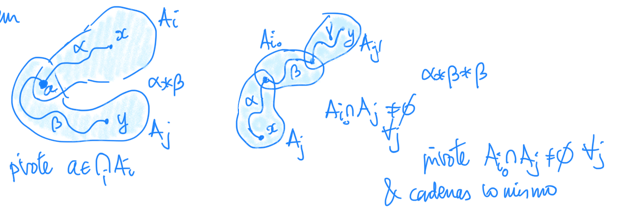
\includegraphics[scale=0.3]{images/dem_pivote_caminos} 
\end{center}
\end{demo}

\begin{prop}[Mantra de la imagen]
Sea $f: X \rightarrow Y$ continua con $X$ conexo por caminos $\Rightarrow f\left( X \right)$ es conexo por caminos. 
\end{prop}
\begin{demo}
\begin{center}
    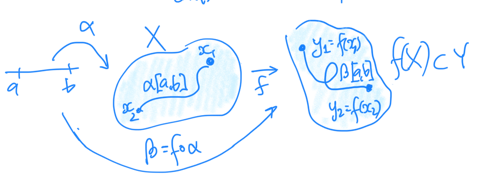
\includegraphics[scale=0.3]{images/dem_imagen_caminos} 
\end{center}
\end{demo}

\begin{prop}[Mantra de la adherencia (¡NO!)]
El seno del topólogo $\Gamma$ = grafo de $\sin \frac{1}{t}$ es conexo por caminos: $\left( a, \sin\frac{1}{a} \right)$ y $\left( b, \sin\frac{1}{b} \right)$ se conectan por el camino evidente, $\alpha\left( t \right) = \left( t, \sin\frac{1}{t} \right),\ a \le t \le b$. Pero, como hemos visto, la adherencia $\overline{\Gamma}$ no es conexa por caminos. 
\end{prop}

\section{Tabla de comportamiento}%
\label{sec:tabla_de_comportamiento_conx_caminos}
%TODO: Fix tabla
\begin{center}    
\begin{tabular}{c | c | c | c | c |}
& Subespacios & Cocientes & Productos & Sumas\\
\hline\\
    Conexión por caminos & $\times$ & \checkmark & \checkmark & $\times$\\
    \hline\\
\end{tabular}
\end{center}

\begin{prop}[Productos]
Sean $\left( x_1, y_1 \right),\ \left( x_2, y_2 \right) \in X \times Y$: 
\[
\begin{rcases}
    \sigma: \left[ a, b \right] \rightarrow X: \begin{cases}
        \sigma\left( a \right) = x_1\\
        \sigma\left( b \right) = x_2
    \end{cases}\\
    \tau: \left[ a, b \right] \rightarrow Y: \begin{cases}
        \tau\left( a \right) = y_1\\
        \tau\left( b \right) = y_2
    \end{cases}
\end{rcases} 
    \Rightarrow \gamma = \left( \sigma, \tau \right) : \left[ a, b \right] \rightarrow X \times Y \begin{cases}
        \gamma\left( a \right) = \left( x_1, y_1 \right)\\
        \gamma\left( b \right) = \left( x_2, y_2 \right)
    \end{cases}  
\]
\end{prop}


\chapter{Componentes conexas por caminos y conexión local por caminos}%
\label{cha:componentes_conexas_por_caminos_y_conexion_local_por_caminos}
\section{Componentes conexas por caminos}%
\label{sec:componentes_conexas_por_caminos}
Todo análogo a las componentes conexas (casi). Sea $X$ espacio topológico.
\begin{defi}
Una componente conexa por caminos (c.c.c) es un subconjunto conexo por caminos maximal.
\end{defi}
\begin{prop}[Descripción]
\begin{enumerate}
    \item La c.c.c de $x \in X$ es $\bigcup_{x \in A} A$ con $A$ conexa por caminos.
    \item Las c.c.c forman una partición de $X$, más fina que la de las c.c.
    \begin{demo}
        Porque conexo por caminos $\Rightarrow$ conexo pero no la inversa.

        \textbf{¡OJO!} Las c.c.c no son necesariamente cerradas. 

        Como contraejemplo de ambas cosas dichas tenemos la adherencia del seno topólogo. 
    \end{demo}
\end{enumerate} 
\end{prop}

\begin{ej}
    $\Gamma$ seno del topólogo y $\overline{\Gamma} = J \cup \Gamma$ son conexos. Tenemos que $\overline{\Gamma}$ es una c.c, mientras que $J$ y $\Gamma$ son dos c.c.c, una cerrada ($J$) y la otra no ($\Gamma$). [Porque $\overline{\Gamma}$ \underline{no} es conexa por caminos]
\end{ej}

\section{Conexión local por caminos}%
\label{sec:conexion_local_por_caminos}
Imitamos sin sorpresa las demostraciones de la conexión local y tenemos:
\begin{defi}
$X$ es \underline{localmente conexo por caminos} si $\forall x \in X,\ \exists \mathcal{B}^x$ base de entornos abiertos conexos por caminos.
\end{defi}
\begin{prop}
$X$ es localmente conexo por caminos $\Leftrightarrow$ c.c.c de un abierto es abierto.
\end{prop}

\underline{Ejercicio}:
Locamente conexo $\Leftrightarrow \forall x \in X,\ \exists \mathcal{V}^x$ base de entornos conexos por caminos. 

\section{Tabla de comportamiento}%
\label{sec:tabla_de_comportamiento_conx_local_caminos}
%TODO: Fix tabla
\begin{center}    
\begin{tabular}{c | c | c | c | c |}
& Subespacios & Cocientes & Productos & Sumas\\
\hline\\
    Conexión local por caminos & $\times$ & \checkmark & \checkmark & \checkmark\\
    \hline\\
\end{tabular}

También vale que las c.c.c del producto son los productos de las c.c.c de los factores.
\end{center}

\section{Relaciones entre las propiedades de conexión}%
\label{sec:relaciones_entre_las_propiedades_de_conexion}
Lo principal es que:
\begin{prop}
Conexo y localmente conexo por caminos $\Rightarrow$ Conexo por caminos.
\end{prop}
\begin{demo}
\begin{itemize}
    \item Conexo $\Rightarrow \forall x, y,\ \exists \text{ cadenas de } x \text{ a } y$.
    \item Localmente conexo por caminos $\Rightarrow$ cadenas de abiertos conexos por caminos $\Rightarrow{\text{Var. pivote}}$ Estas cadenas son conexas por caminos.
\end{itemize}
Por tanto, $\exists$ camino de $x$ a $y$.
\end{demo}
\begin{obs}
    Esta es la demostración de que un abierto conexo de $\mathbb{R}_u^n$ lo es por poligonales (se usan cadenas de bolas).
\end{obs}

\begin{obs}[Resumen]
Por especificar todas las posibilidades:
%TODO: Imagen
\begin{center}
    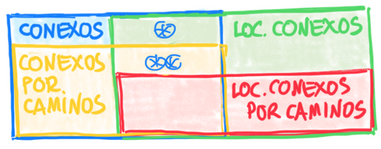
\includegraphics[scale=0.3]{images/resumen_conx} 
\end{center}
\end{obs}

\underline{Ejercicio}: Contraejemplos. Los menos fáciles son $*$ y $**$ 

\chapter{Homotopía}%
\label{cha:homotopia}
\section{Conceptos fundamentales}%
\label{sec:conceptos_fundamentales}
\begin{defi}
Una \underline{homotopía} es una aplicación continua $H : Y \times \left[ 0, 1 \right] \rightarrow X$:
\begin{enumerate}
    \item $H_s : Y \rightarrow X: y \mapsto H\left( y, s \right),\ H \equiv \{H_s: 0 \le s \le 1\}$ familia uniparamétrica de aplicaciones.
    \item Siendo $f = H_0$ y $g = H_1$:
    \[
    \begin{cases}
        H_s : f \simeq g \text{ homotopía entre } f \text{ y } g\\
        H \text{ deformación continua de } f \text{ a } g
    \end{cases} \boxed{\text{El problema: cuándo } f \simeq g} 
    \]

    \item $f \simeq g$ relación de equivalencia:
    \begin{itemize}
        \item $f \simeq f$ vía $H_s \equiv f$.
        \item $H_s : f \simeq g \Rightarrow H_{1 - s} : g \simeq f$.
        \item $\begin{rcases}
            F_s : f \simeq g\\
            G_s: g \simeq h
        \end{rcases} \Rightarrow H_s = \begin{cases}
            F_{2s},\ 0 \le s \le 1/2\\
            G_{2s - 1}\ 1/2 \le s \le 1
        \end{cases}: f \simeq h$
        \begin{demo}
            Continuidad: $\begin{cases}
            F_{2(1/2)} = F_1 = g\\
            G_{2(1/2) - 1} = G_0 = g
            \end{cases}$
        \end{demo}
    \end{itemize}
\end{enumerate}
\end{defi}

\begin{prop}
$X$ conexo por caminos, $f, g: Y \rightarrow X$ constantes $\Rightarrow f \simeq g$.
\end{prop}
\begin{demo}
$\exists \sigma: \left[ 0, 1 \right] \rightarrow X,\ \sigma\left( 0 \right) = f\left( y_0 \right)$ y $\sigma\left( 1 \right) = g\left( y_0 \right) \Rightarrow H_s \equiv \sigma\left( s \right) : \begin{cases}
    H_0 \equiv \sigma\left( 0 \right) = f\left( y_0 \right) \equiv f\\
    H_1 \equiv \sigma\left( 1 \right) = g\left( y_0 \right) \equiv g
\end{cases}$
\end{demo}

\begin{defi}
$f: Y \rightarrow X$ es \underline{nulhomótopa} si $f \simeq $ constante, \underline{esencial} en caso contrario.
\end{defi}

\begin{theo}[Problema esencial. Hopf.]
(1932) $\exists f : \mathbb{S}^3 \rightarrow \mathbb{S}^2$ esencial con $\mathbb{S}^3 \subset \mathbb{R}^4 = \mathbb{C}^2$ y $\mathbb{S}^2 \subset \mathbb{R}^3 = \mathbb{R} \times \mathbb{C}: \left( z, z' \right) \mapsto \left( \lVert z \rVert^2 - \lVert z' \rVert^2, 2 z z'\right) $ 
\end{theo}

\section{Concepto relativo}%
\label{sec:concepto_relativo}
\begin{defi}
$H: Y \times \left[ 0, 1 \right] \rightarrow X$ es relativa a $A \subset Y$ si $H_s\left( a \right) = H_0\left( a \right),\ \forall a \in A,\ \forall s$.
\end{defi}

\begin{prop}
$H$ relativa a $A,\ f = H_0,\ g = H_1 \Rightarrow f|_A = g|_A$. Notación: $H_s = f \stackrel{A}{\simeq} g$ (Relación de equivalencia).
\end{prop}

\begin{ej}[Fundamentales. Interpolación]
\begin{enumerate}
    \item $f, g: Y \rightarrow X \subset \mathbb{R}^n$ convexo $\Rightarrow\exists H_s = \left( 1 - s \right) f + sg: f \simeq g$.
    \begin{demo}
        Pues por convexidad $H_s\left( y \right) \in \underbrace{\left[ f\left( y \right), g\left( y \right) \right] \subset X}_{\text{\textbf{cond. crucial!}}}$.
    \end{demo}
    $f\left( a \right) = g\left( a \right) \Rightarrow H_s\left( a \right) = f\left( a \right) = g\left( a \right) \Rightarrow H_s$ es relativa a $A = \{f = g\}$.

    \item $f: Y \rightarrow X \subset \mathbb{R}^n$ estrellado verp?, $x_0,\ \left[ x, x_0 \right] \subset X,\ \forall x \in X \Rightarrow H_s = \left( 1 - s \right)f + sx_0: f \simeq x_0$ (relativa a $A = f^{-1}\left( x_0 \right)$).

    \item Variante en $\mathbb{S}^n$:
    %TODO: Imagen
    \begin{center}
        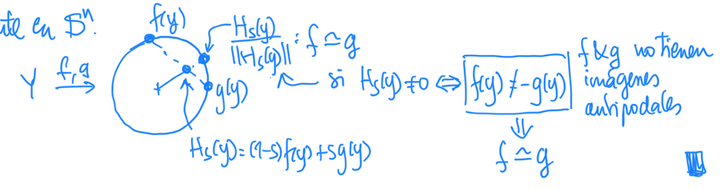
\includegraphics[scale=0.3]{images/ej_fund_interp_3} 
    \end{center}
\end{enumerate} 
\end{ej}

\section{Contractibilidad}%
\label{sec:contractibilidad}
\begin{defi}
$X$ es \underline{contráctil} si $id: X \rightarrow X$ es nulhomótopa: $\exists H_s : id \simeq x_0$.

Y \underline{fuertemente contrátil} si $\exists H_s : id \stackrel{x_0}{\simeq} x_0$ (homótopa relativa a $\{x_0\}$)
\end{defi}

\begin{obs}
Los ejemplos son difíciles, pero son cosas distintas.
\end{obs}

\begin{ej}
    $X \subset \mathbb{R}^n$ estrellado verp? $x_0 \Rightarrow$ fuertemente contráctil
    \begin{demo}
        $H_s = \left( 1 - s \right) id + sx_0$.
    \end{demo}
\end{ej}

\begin{prop}
\begin{enumerate}
    \item Si $X$ es contrátil $\Rightarrow$ es conexo por caminos.
    \item Si $X$ es contráctil $\Rightarrow \begin{cases}
        \forall f: Y \rightarrow X \text{ nulhomótopa.}\\
        \forall g: X \rightarrow Z \text{ nulhomótopa.} 
    \end{cases} $
\end{enumerate}
\end{prop}
\begin{demo}
\begin{enumerate}
    \item $H_s: id \simeq x_0 \Rightarrow S \mapsto H_s\left( x_0 \right)$ camino de $x$ a $x_0$.
    \item $H_s: id \simeq x_0 \begin{cases}
        H_s \circ f: f \simeq x_0\\
        g \circ H_s: g \simeq g\left( x_0 \right) 
    \end{cases} $
\end{enumerate}
\end{demo}
\begin{obs}
Pocos espacios son contráctiles, pero no es inmediato verlo.
\end{obs}

\chapter{Homotopía de caminos}%
\label{cha:homotopia_de_caminos}
\section{El concepto básico}%
\label{sec:el_concepto_basico}
\begin{defi}
$\sigma, \tau: \left[ a, b \right] \rightarrow X$ son homótopos \underline{con extremos fijos} si $\exists H_s: \sigma \simeq \tau$ relativa a $\{a, b\}$: 
\[
\begin{cases}
    H_s\left( a \right) = \sigma\left( a \right) = \tau\left( a \right)\\
    H_s\left( b \right) = \sigma\left( b \right) = \tau\left( b \right) 
\end{cases}\forall s
\]
%TODO: Imagen
\begin{center}
    \includegraphics[scale=0.3]{images/def_homp_ext_fijos} 
\end{center}
\end{defi}

\begin{obs}
Es un problema de \underline{extensión}: 

Definir $H$ en el cuadrado $\left[ a, b \right] \times \left[ 0, 1 \right]$ con valor determinado en su borde.
%TODO: Imagen
\begin{center}
    \includegraphics[scale=0.3]{images/obs_problema_ext} 
\end{center}
\end{obs}

\section{Simple-conexión}%
\label{sec:simple_conexion}
\begin{defi}
$X$ es \underline{simplemente conexo} si cumple las siguientes condiciones equivalentes:
\begin{enumerate}
    \item $\forall \sigma, \tau: \left[ a, b \right] \rightarrow X$ con iguales extremos son homótopos con extremos fijos.
    \item $\forall f: \mathbb{S}' \rightarrow X$ se extiende al disco interior de la circunferencia.
\end{enumerate}
\end{defi}
\begin{demo}
    Colapsando dos lados de un cuadrado $\xrightarrow{\pi}$ disco con dos puntos en la circunferencia unidos por dos ceros $\alpha, \beta$.

    \item 1. $\Rightarrow$ 2.) 
    \begin{align*}
        f: \mathbb{S}^1 \rightarrow X &\Rightarrow f \circ \pi \begin{cases}
            \alpha \rightarrow \text{ camino } \sigma\\
            \beta \rightarrow \text{ camino } \tau
        \end{cases}\\
        &\Rightarrow \exists H \text{ con extremos fijos } \Rightarrow \text{ compatible con } \pi \\
        &\Rightarrow H \text{ pasa al cociente por } \pi \text{, dando } F.
    .\end{align*}

    \item 2. $\Rightarrow$ 1.) Dos caminos $\sigma, \tau$ con extremos $p, q$ definen $f$ en la circunferencia y su extensión $F$ al disco define la homotopía $H = F \circ \pi$.
\end{demo}

\begin{ej}
Los conjuntos convexos son simplemente conexos. ¿Los estrellados?
\end{ej}

\section{Esferas \texorpdfstring{$\mathbb{S}^n,\ n \ge 2$}{Sn, n >= 2}}%
\label{sec:esferas_s_n}
\begin{prop}
$\mathbb{S}^n : \{x_1^2 + \ldots + x_{n + 1}^2 = 1\} \subset \mathbb{R}^{n + 1}$ es simplemente conexo ($n \ge 2$).
\end{prop}
\begin{demo}
$\sigma, \tau: \left[ a, b \right] \rightarrow \mathbb{S}^n,\ \sigma\left( a \right) = \tau\left( a \right) = p,\ \sigma\left( b \right) = \tau\left( b \right) = q$.
\[
\exists c, -c \in \mathbb{S}^n\setminus \{p, 1\}\; \land \;\begin{rcases}
   U = \mathbb{S}^n \setminus \{c\} \stackrel{\text{homeo.}}{\approx} \mathbb{R}^n\\
   V = \mathbb{S}^n \setminus \{-c\} \stackrel{\text{homeo.}}{\approx} \mathbb{R}^n
\end{rcases} \text{proyección estéreo.}  
\]
\begin{enumerate}
    \item $\left[ a, b \right] \subset \sigma^{-1}U \cup \sigma^{-1}V \xRightarrow{\text{comp.}} \exists a = t_0 < t_1 < \ldots < t_r = 1: \sigma\left[ t_{i - 1}, t_1 \right] \begin{cases}
        \subset U\\
        \subset V
    \end{cases}$ dónde $\sigma\left[ t_{i - 1}, t_i \right]$ es la traza de $\sigma_i = \sigma|_{\left[ t_{i - 1}, t_i \right]}$.

    \item Si dos consecutivos están en el mismo $U$ ó $V$, eliminamos la juntura común $\Rightarrow$ al atravesar una juntura $t_k$ cambiamos de $U$ a $V$ ó viceversa, en particular, $x_k = \sigma\left( t_k \right) \in U \cap V \approx \mathbb{R}^n \setminus \{\text{punto}\}$, que es conexo por caminos, o bien, nos quedamos sin junturas y $\sigma\left[ a, b \right] \subset U$ ó $V$.

    \item Consideramos los trozos en $V$ (incluido que $\sigma\left[ a, b \right] \subset V$ porque no hay ya junturas)
    \begin{center}
        \includegraphics[scale=0.3]{images/esferas_sn_3} 
    \end{center}
    \begin{itemize}
        \item[(*)]
        \begin{align*}
            \sigma\left( t_{i - 1} \right), \sigma\left( t_i \right) \in U \cap V &\approx \mathbb{R}^n \setminus \{\text{punto}\} \text{ conexo por caminos}\\
            &\Rightarrow \exists \sigma_i^*: \left[ t_{i - 1}, t_i \right] \rightarrow U\cap V \subset V \text{ mismos extremos que } \sigma_i
        .\end{align*}

        \item[(**)] $V \approx \mathbb{R}^n$ convexo $\Rightarrow \exists H_s^i: \sigma_i \simeq \sigma_i^*$ en $V$ con extremos fijos. ¡Ojo! $\boxed{\sigma_i^*: \left[ t_{i - 1}, t_i \right] \rightarrow U}$.
    \end{itemize}

    \item Pegando a trozos homotopías en $\mathbb{S}^n$:
    \[
    \begin{cases}
        \sigma\left[ t_{i_1}, t_i \right] \subset U \Rightarrow H_s^i \equiv \sigma_i = \sigma_i^*: \left[ t_{i - 1}, t_i \right] \rightarrow U \subset \mathbb{S}^n\\
        \sigma\left[ t_{i_1}, t_i \right] \subset V \xRightarrow{3} H_s^i : \sigma_i \simeq \sigma_i^*: \left[ t_{i - 1}, t_i \right] \rightarrow V \subset \mathbb{S}^n
    \end{cases} \Rightarrow \sigma \simeq \sigma^* 
    \]
    Homótopos en $\mathbb{S}^n$ con extremos fijos, pero $\sigma^*\left[ a, b \right] \subset U$.

    \item Igual, $\exists H_s: \tau \simeq \tau^*$ homotopía en $\mathbb{S}^n$ con extremos fijos, pero $\tau^*\left[ a, b \right] \subset U$.
\end{enumerate}
En conclusión: $\sigma^* \simeq \tau^*$ en $U \left( \approx \mathbb{R}^n \right)$ con extremos fijos $\Rightarrow \sigma \simeq \sigma^* \simeq \tau^* \simeq \tau$ con extremos fijos.
\end{demo}

\chapter{El grupo fundamental}%
\label{cha:el_grupo_fundamental}

\chapter{Retractos}%
\label{cha:retractos}

\chapter{Recubridores}%
\label{cha:recubridores}

\chapter{Cálculos mediante recubridores}%
\label{cha:calculos_mediante_recubridores}

\chapter{Aplicaciones en dimensión 2}%
\label{cha:aplicaciones_en_dimension_2_}

\chapter{Más aplicaciones por el mismo precio}%
\label{cha:mas_aplicaciones_por_el_mismo_precio}

\chapter{Superficies}%
\label{cha:superficies}

\chapter{Clasificación de superficies}%
\label{cha:clasificacion_de_superficies}

\chapter{Grande finale}%
\label{cha:grande_finale}




\end{document}
